% sage_latex_guidelines.tex V1.10, 24 June 2016

\documentclass[Afour,sageh,times]{sagej}

\usepackage{moreverb,url}

\usepackage[colorlinks,bookmarksopen,bookmarksnumbered,citecolor=red,urlcolor=red]{hyperref}

\newcommand\BibTeX{{\rmfamily B\kern-.05em \textsc{i\kern-.025em b}\kern-.08em
T\kern-.1667em\lower.7ex\hbox{E}\kern-.125emX}}

% customizations
\usepackage{tikz}
\usepackage{booktabs}
\usepackage{tabularx}
\newcolumntype{Y}{>{\raggedright\arraybackslash}X}
\usepackage{array}
\newcommand{\ra}[1]{\renewcommand{\arraystretch}{#1}}

\def\volumeyear{2017}

\begin{document}

\runninghead{Harmon et~al.}

\title{Tangible Landscape}

\author{Brendan A Harmon\affilnum{1,2}, Anna Petrasova\affilnum{1}, Vaclav Petras\affilnum{1}, Helena Mitasova\affilnum{1}, and Ross Meentemeyer\affilnum{1}}

\affiliation{\affilnum{1}Center for Geospatial Analytics, North Carolina State University, USA\\
\affilnum{2}College of Design, North Carolina State University, USA}

\corrauth{Brendan A Harmon, 
Center for Geospatial Analytics,
North Carolina State University,
Raleigh, NC 27615, USA.}

\email{brendan.harmon@gmail.com}

\begin{abstract}
\ldots
\end{abstract}

\keywords{\ldots}

\maketitle


\clearpage

% ---------------------------- TEMPLATE ---------------------------- 

%\begin{figure*}
%%\setlength{\fboxsep}{0pt}%
%%\setlength{\fboxrule}{0pt}%
%\begin{center}
%\end{center}
%\caption{...}
%\label{F1}
%\end{figure*}

% ---------------------------- AUX ---------------------------- 

\begin{table*}[h]
\small\sf\centering
\caption{Bivariate scatterplots of elevation values}
\ra{1.3}
\begin{tabular}{m{0.07\textwidth} m{0.28\textwidth} m{0.28\textwidth} m{0.28\textwidth}}
\toprule
& \multicolumn{1}{c}{Digital} & \multicolumn{1}{c}{Analog}  & \multicolumn{1}{c}{Tangible}\\
\midrule \\
Mean & 
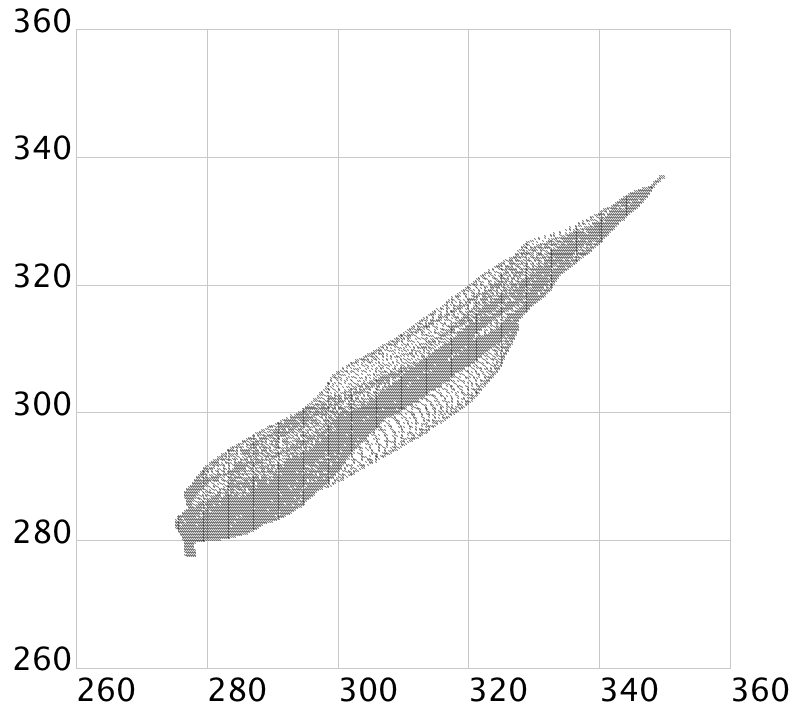
\includegraphics[width=0.28\textwidth]{images/bivariate_scatterplots/dem_1.png} &
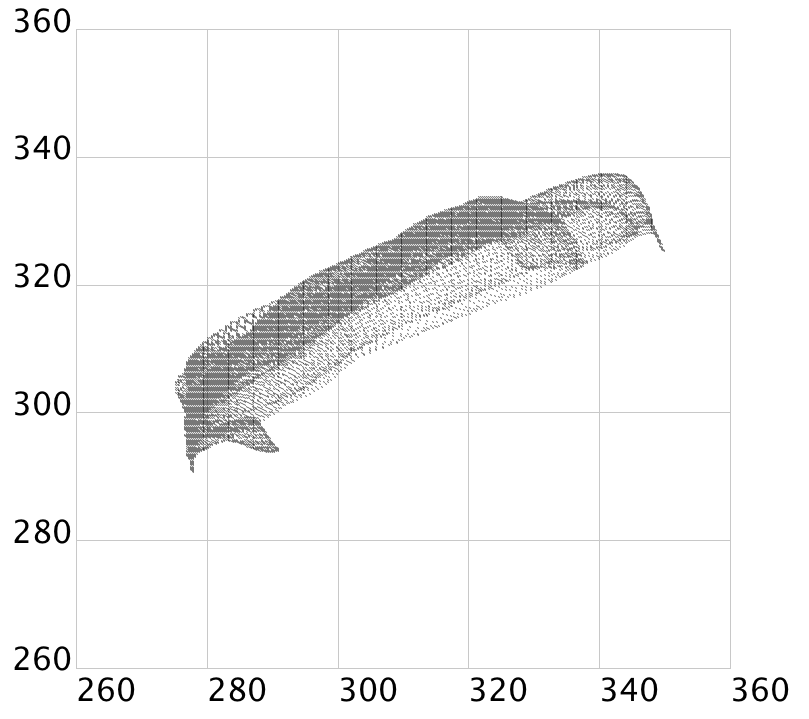
\includegraphics[width=0.28\textwidth]{images/bivariate_scatterplots/dem_2.png} &
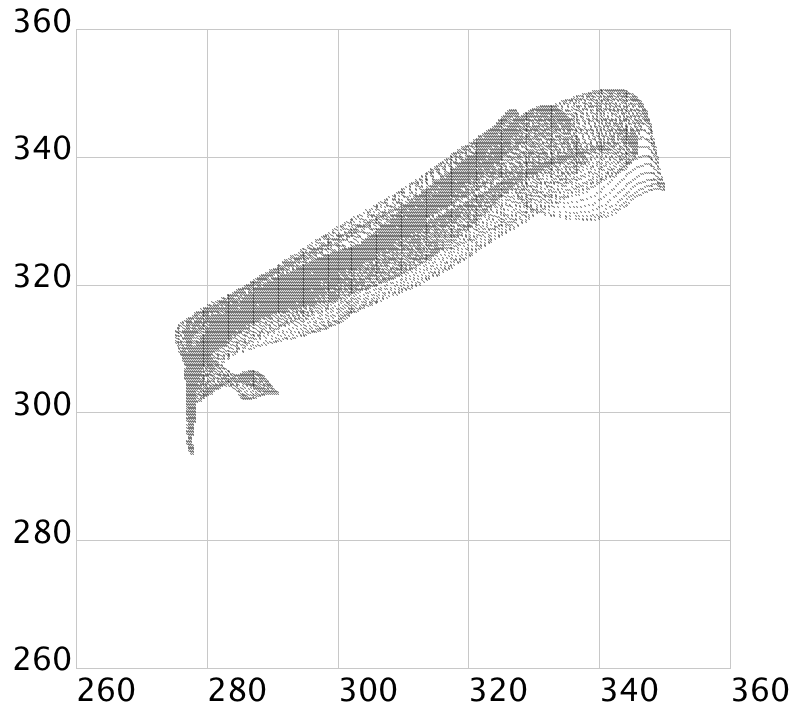
\includegraphics[width=0.28\textwidth]{images/bivariate_scatterplots/dem_3.png}\\
& \multicolumn{1}{c}{Reference} & \multicolumn{1}{c}{Reference} & \multicolumn{1}{c}{Reference} \\
\\
\bottomrule
\end{tabular}
\label{table:scatterplots} 
\end{table*}

%% landform legend
%\begin{figure*}[h]
%\begin{center}
%		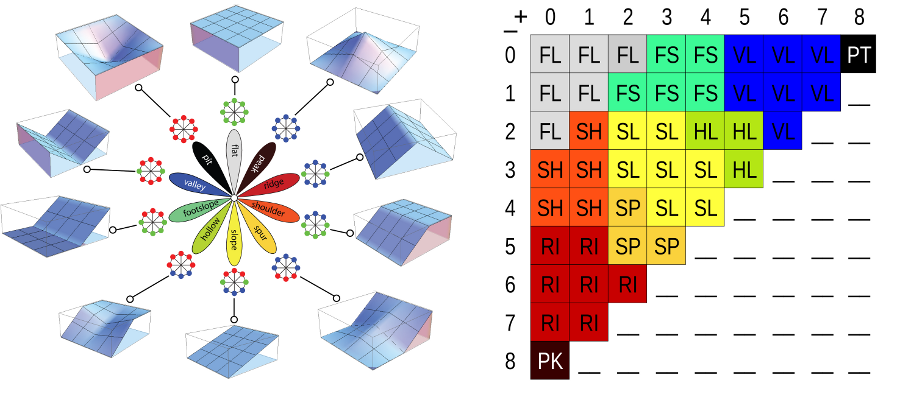
\includegraphics[width=0.9\textwidth]{images/geomorphons_legend.png}
%	\caption{Landforms identified by \textit{r.geomorphon} --
%		1)~flat, 
%		2)~peak, 
%		3)~ridge, 
%		4)~shoulder, 
%		5)~spur, 
%		6)~slope, 
%		7)~hollow, 
%		8)~footslope, 
%		9)~valley, and
%		10)~depression.
%		Source: \cite{r.geomorphon}.}
%	\label{fig:geomorphons}
%\end{center}
%\end{figure*}

% ---------------------------- TREE ---------------------------- 

\begin{figure*}[h]
\begin{center}
\resizebox {\textwidth} {!} {
\begin{tikzpicture}[grow = right,
	level 1/.style={sibling distance=12 em},
	level 2/.style={sibling distance=6 em},
	level distance = 14em,
	every node/.style = {shape=rectangle, 
		rounded corners,
		draw, 
		font=\footnotesize\sffamily,
		align=center,
		top color=white,
		bottom color=white}]
\node {Participants \\ 
	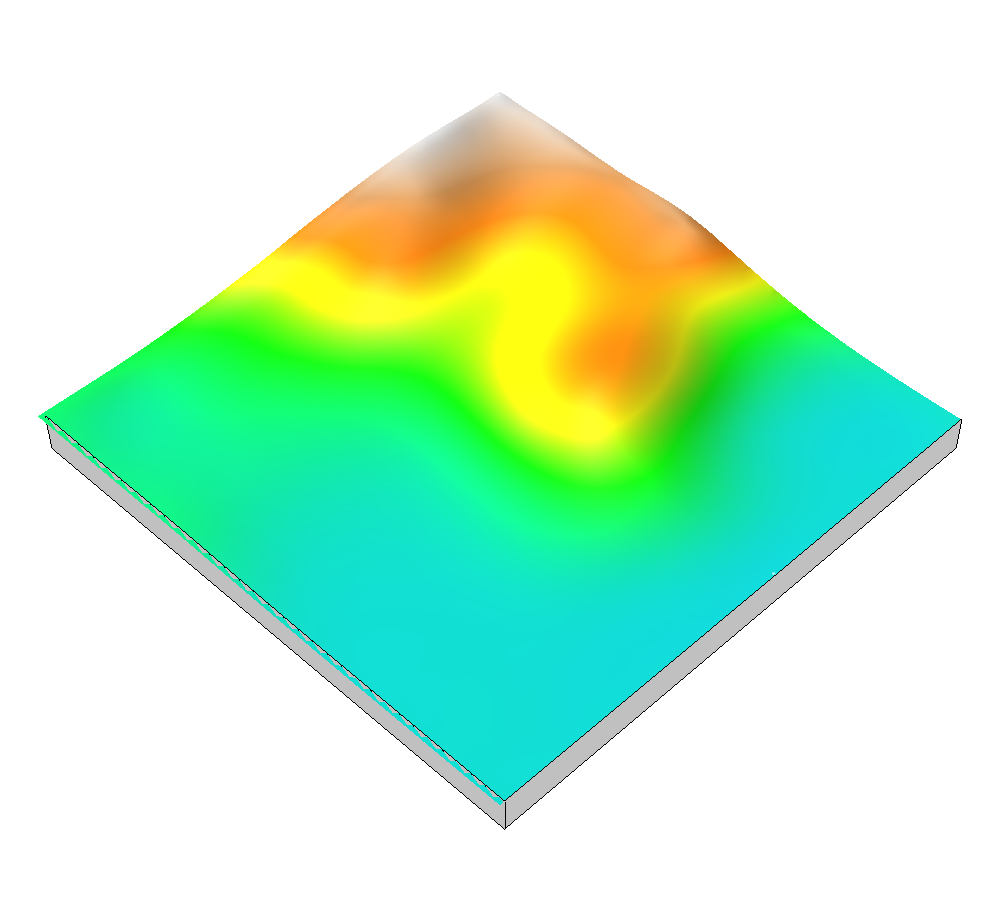
\includegraphics[width=0.08\textwidth]{images/render_3d/participants/mean_dem_1.png}
	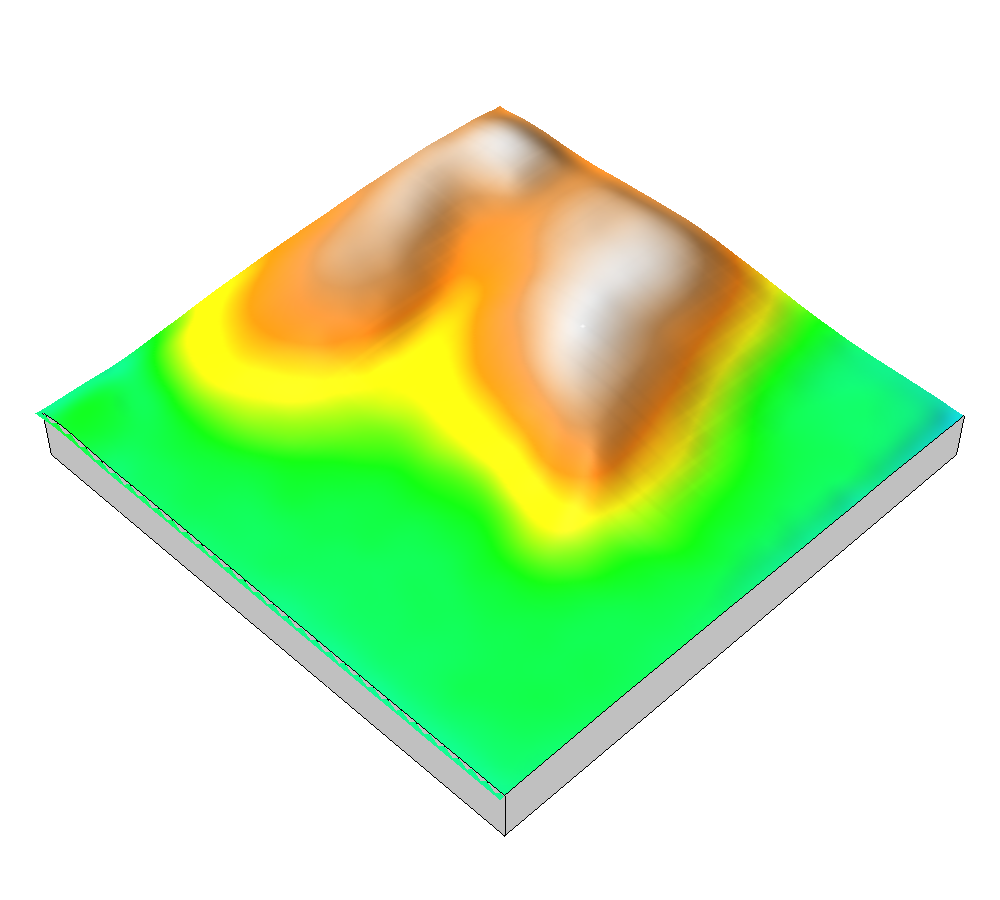
\includegraphics[width=0.08\textwidth]{images/render_3d/participants/mean_dem_2.png}
	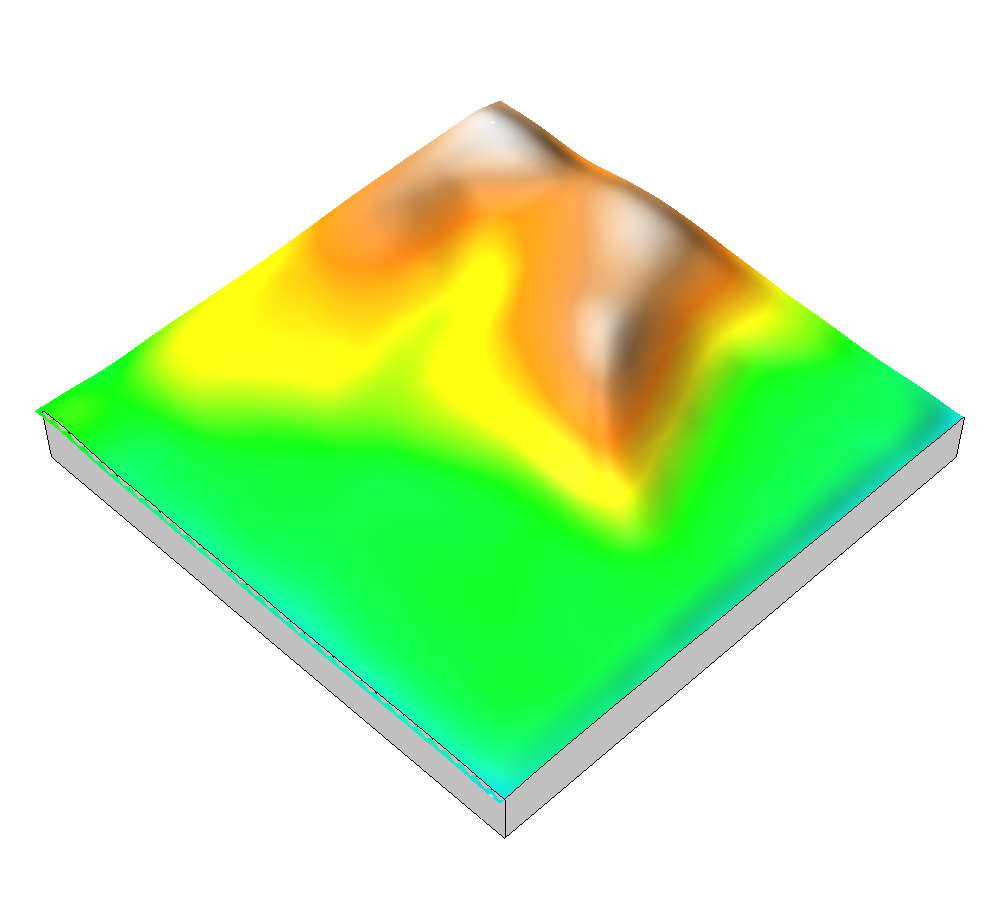
\includegraphics[width=0.08\textwidth]{images/render_3d/participants/mean_dem_3.png} \\
	\makebox[0.08\textwidth][c]{\scriptsize Digital}
	\makebox[0.08\textwidth][c]{\scriptsize Analog}
	\makebox[0.08\textwidth][c]{\scriptsize Tangible}
	}
	child { node {Students \\ 
		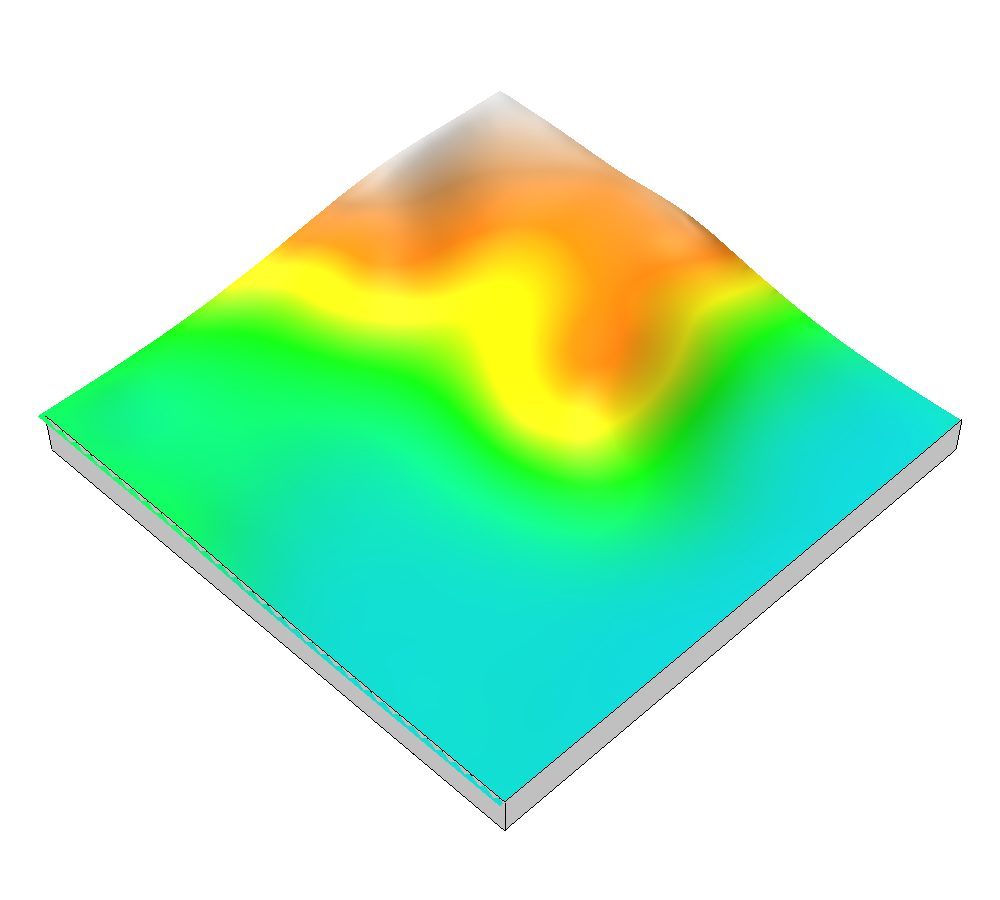
\includegraphics[width=0.08\textwidth]{images/render_3d/students/mean_dem_1.png}
		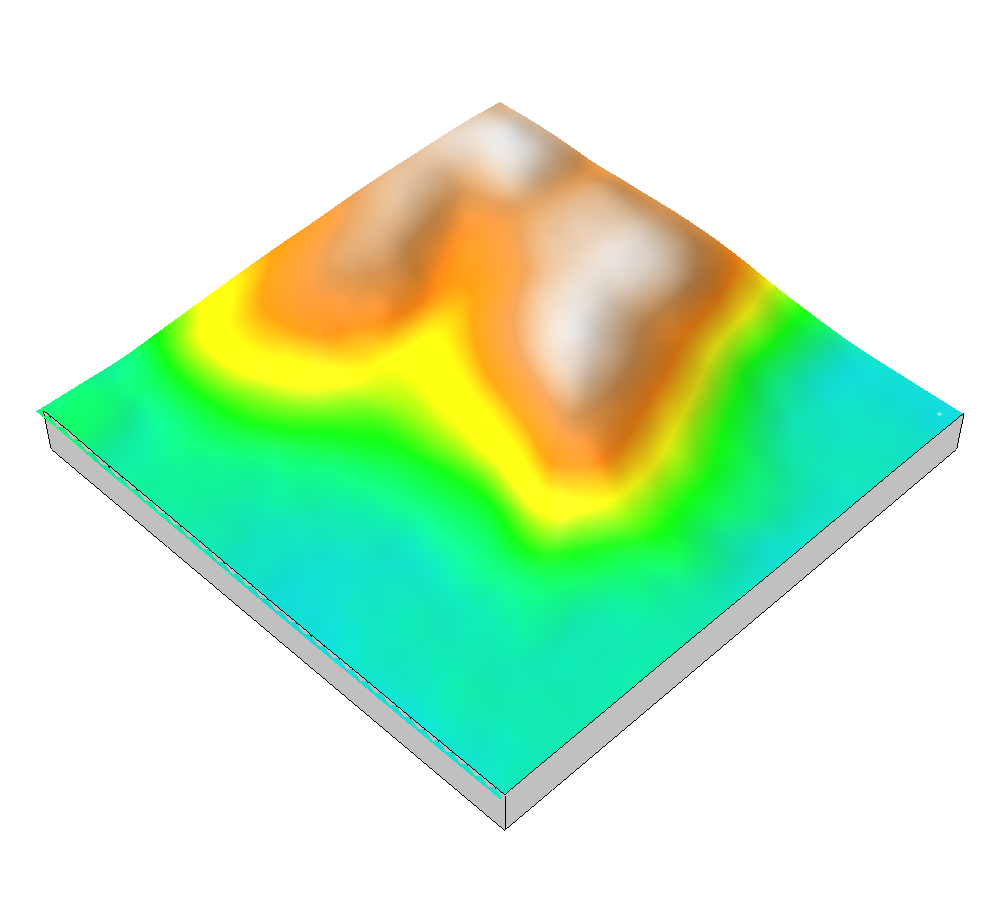
\includegraphics[width=0.08\textwidth]{images/render_3d/students/mean_dem_2.png}
		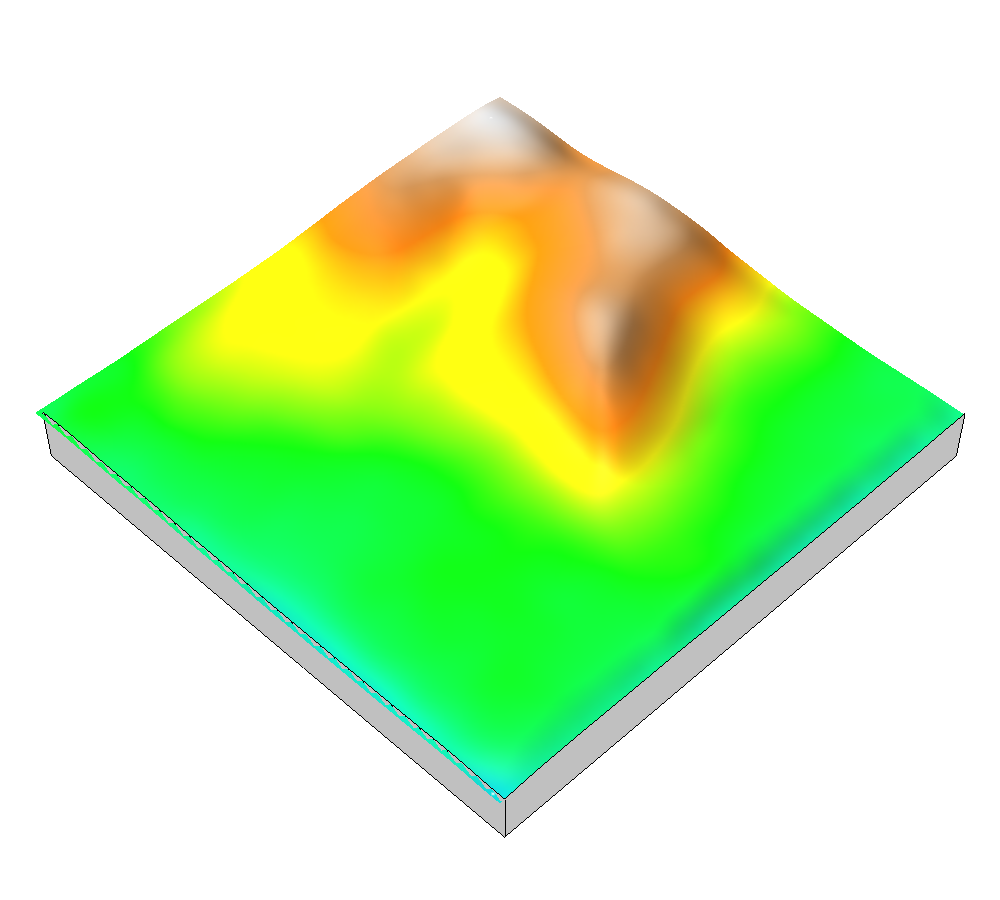
\includegraphics[width=0.08\textwidth]{images/render_3d/students/mean_dem_3.png}
		}
		child { node {Landscape architecture \\ 
			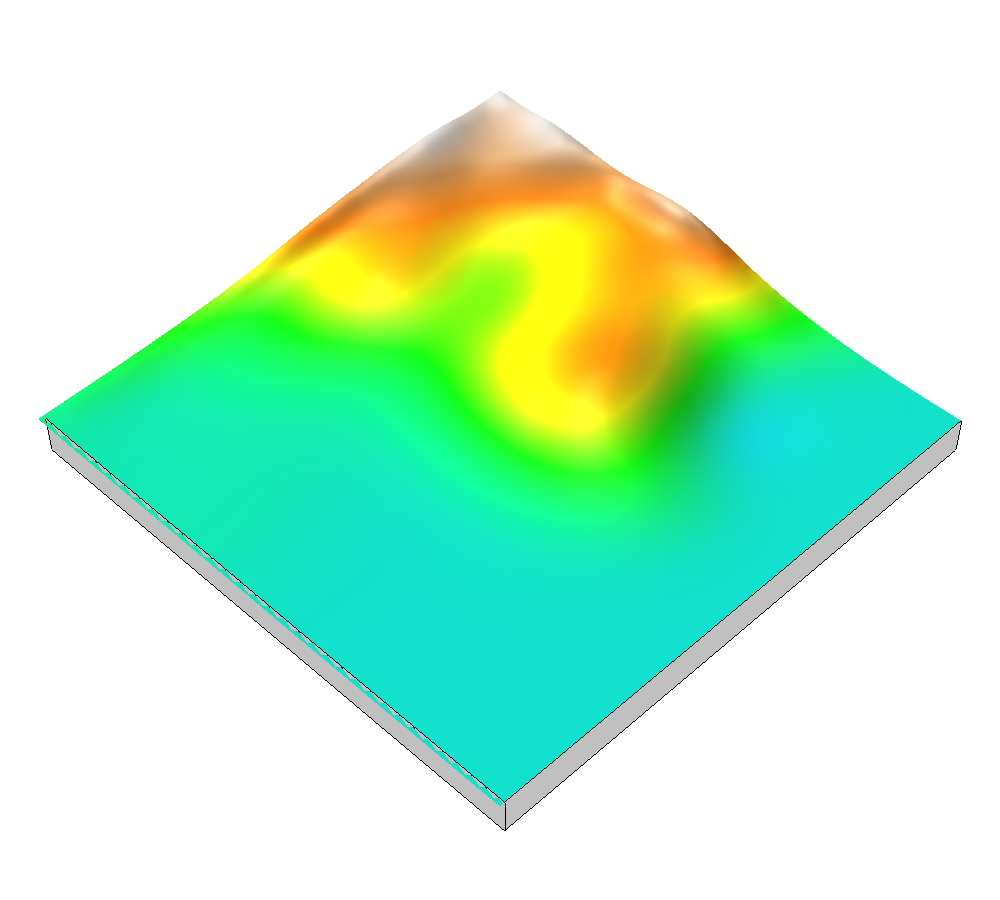
\includegraphics[width=0.08\textwidth]{images/render_3d/landscape_students/mean_dem_1.png}
			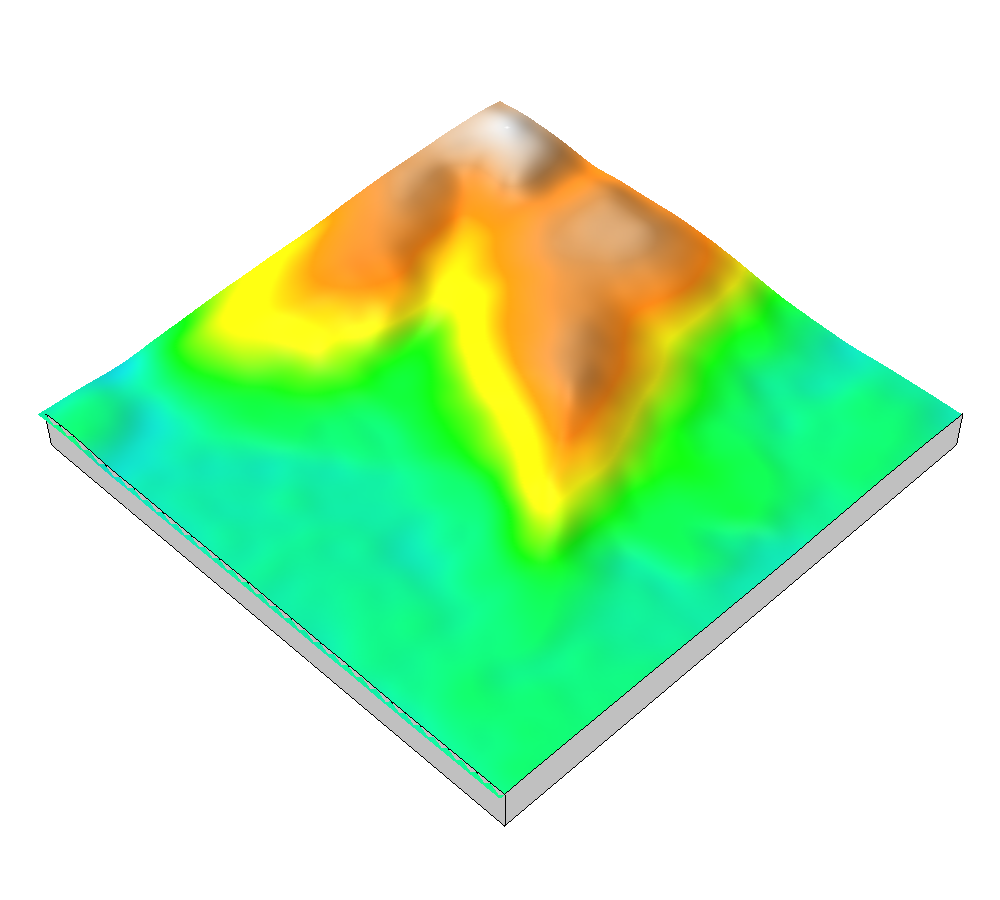
\includegraphics[width=0.08\textwidth]{images/render_3d/landscape_students/mean_dem_2.png}
			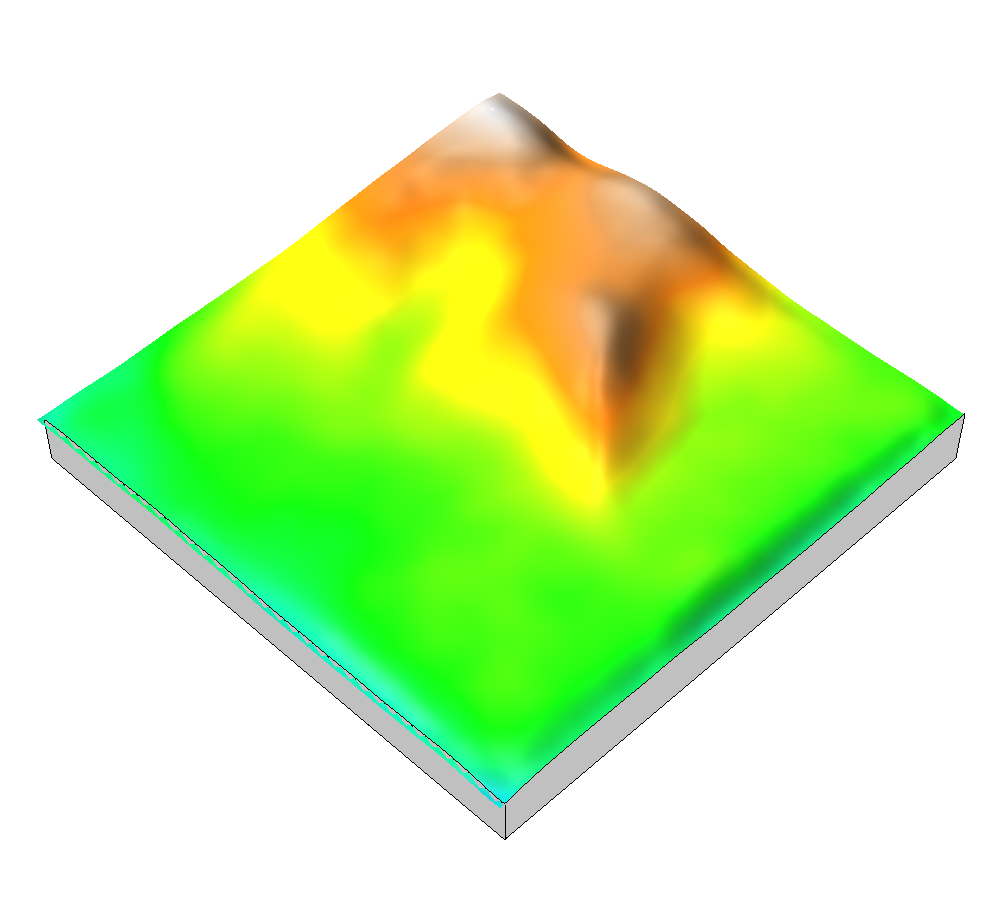
\includegraphics[width=0.08\textwidth]{images/render_3d/landscape_students/mean_dem_3.png}
			}
			}
		child { node {GIS \\ 
			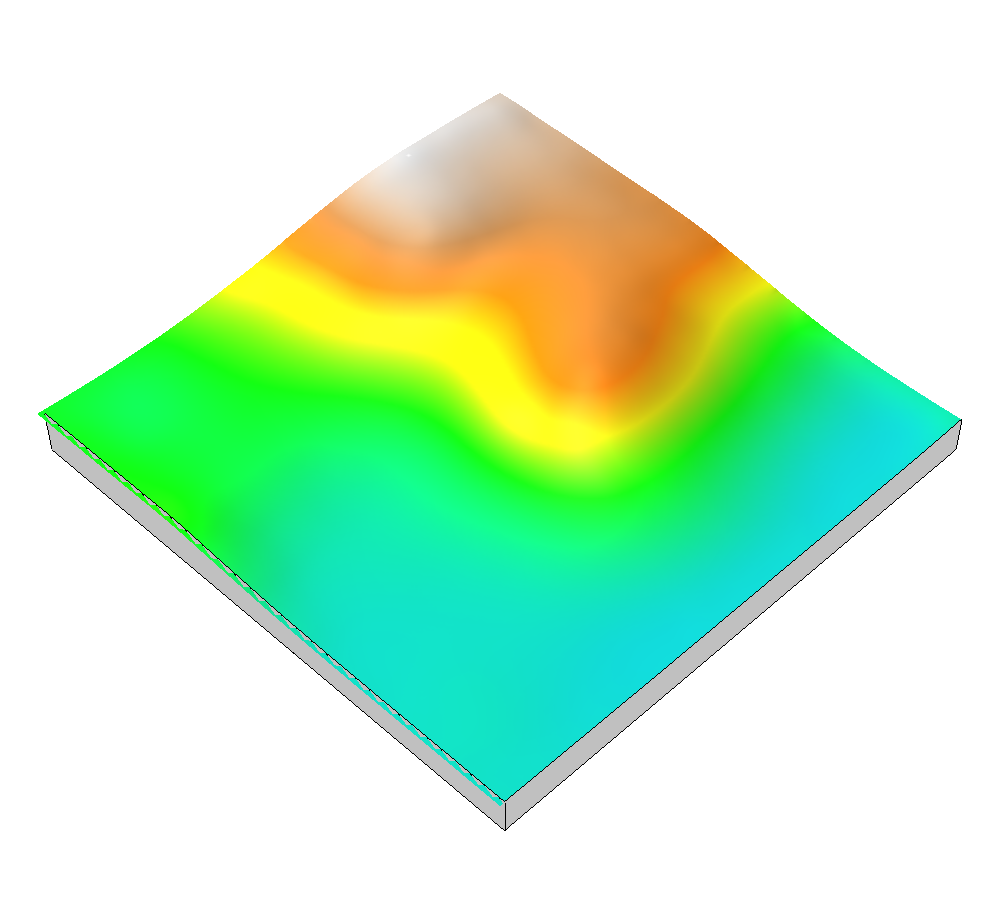
\includegraphics[width=0.08\textwidth]{images/render_3d/gis_students/mean_dem_1.png}
			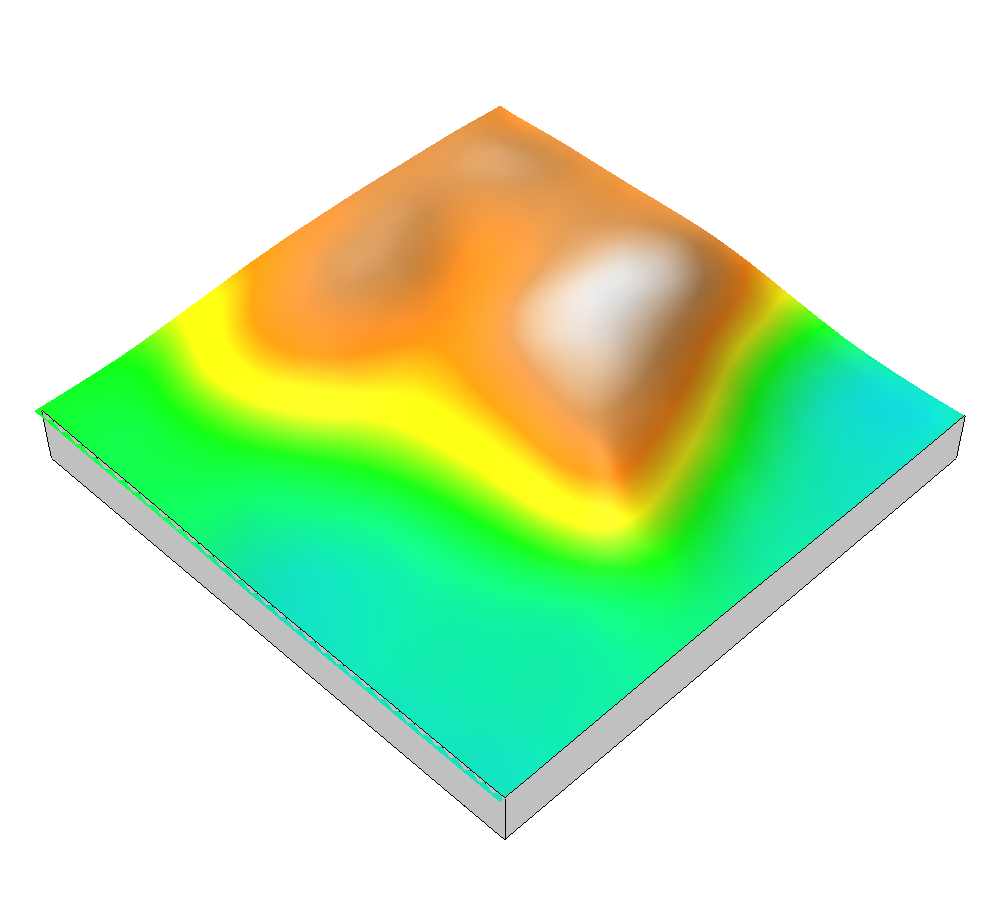
\includegraphics[width=0.08\textwidth]{images/render_3d/gis_students/mean_dem_2.png}
			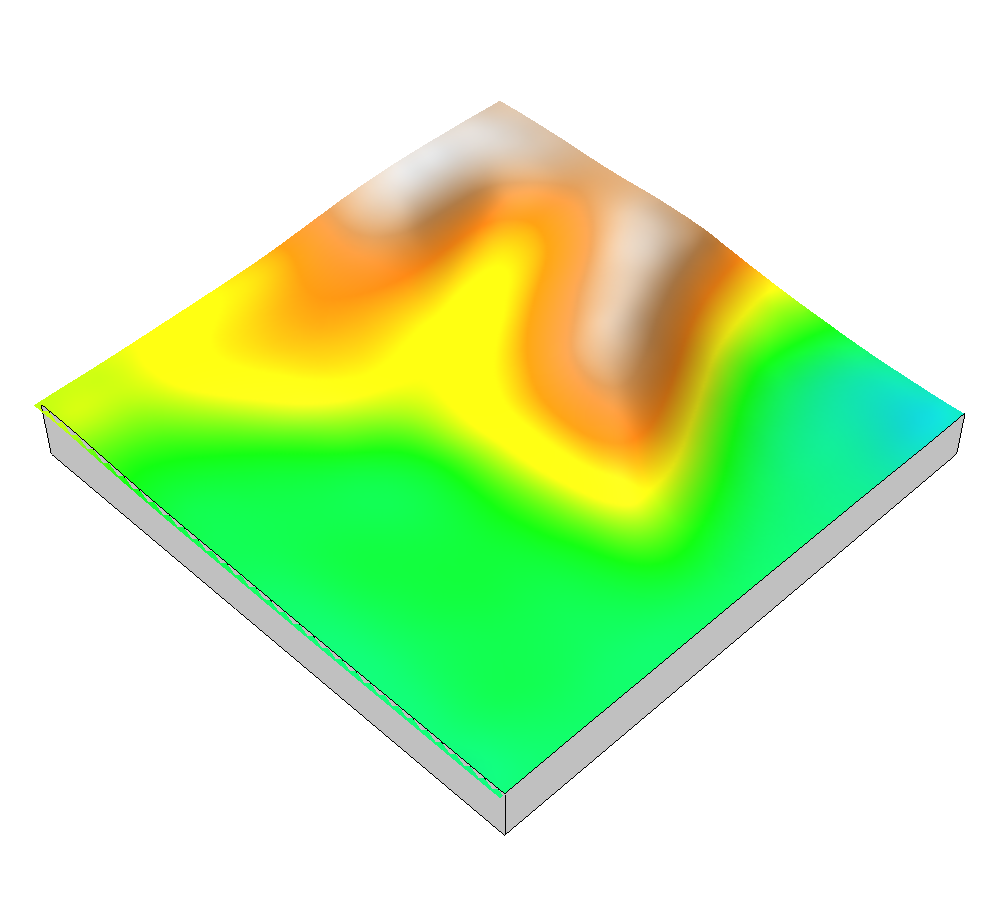
\includegraphics[width=0.08\textwidth]{images/render_3d/gis_students/mean_dem_3.png}
			}
			}
		}
	child { node {Professionals \\ 
		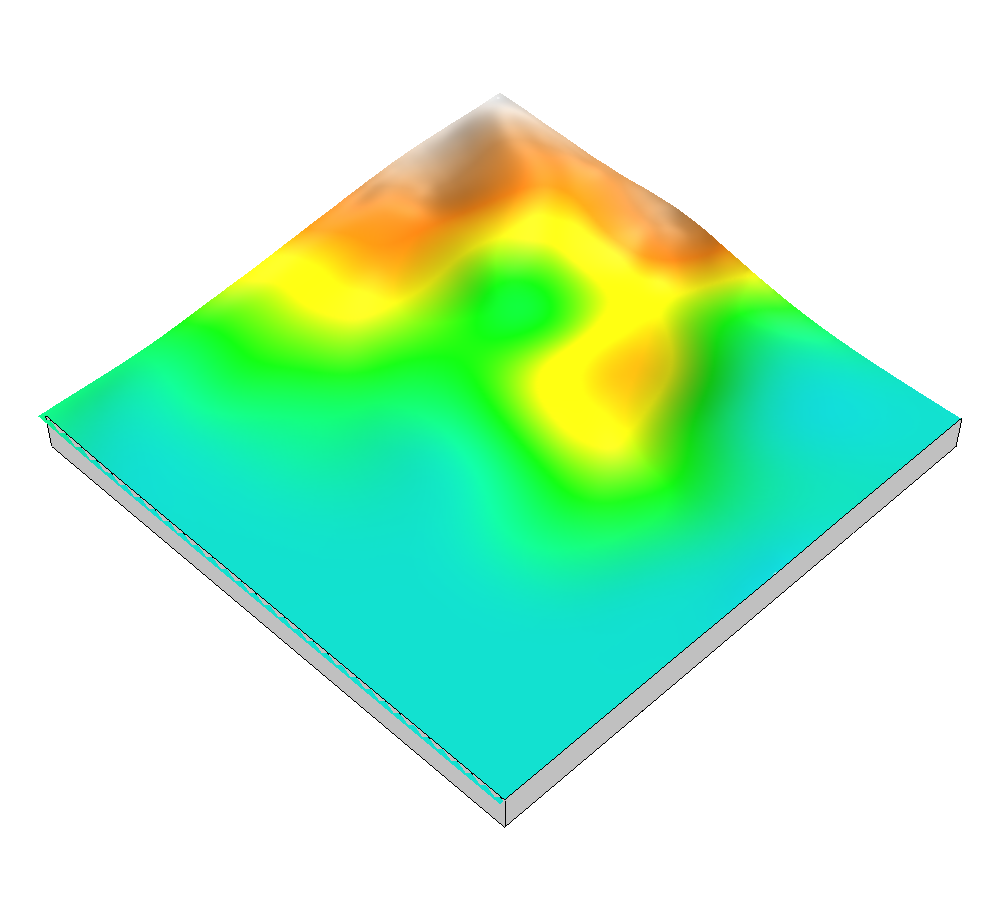
\includegraphics[width=0.08\textwidth]{images/render_3d/professionals/mean_dem_1.png}
		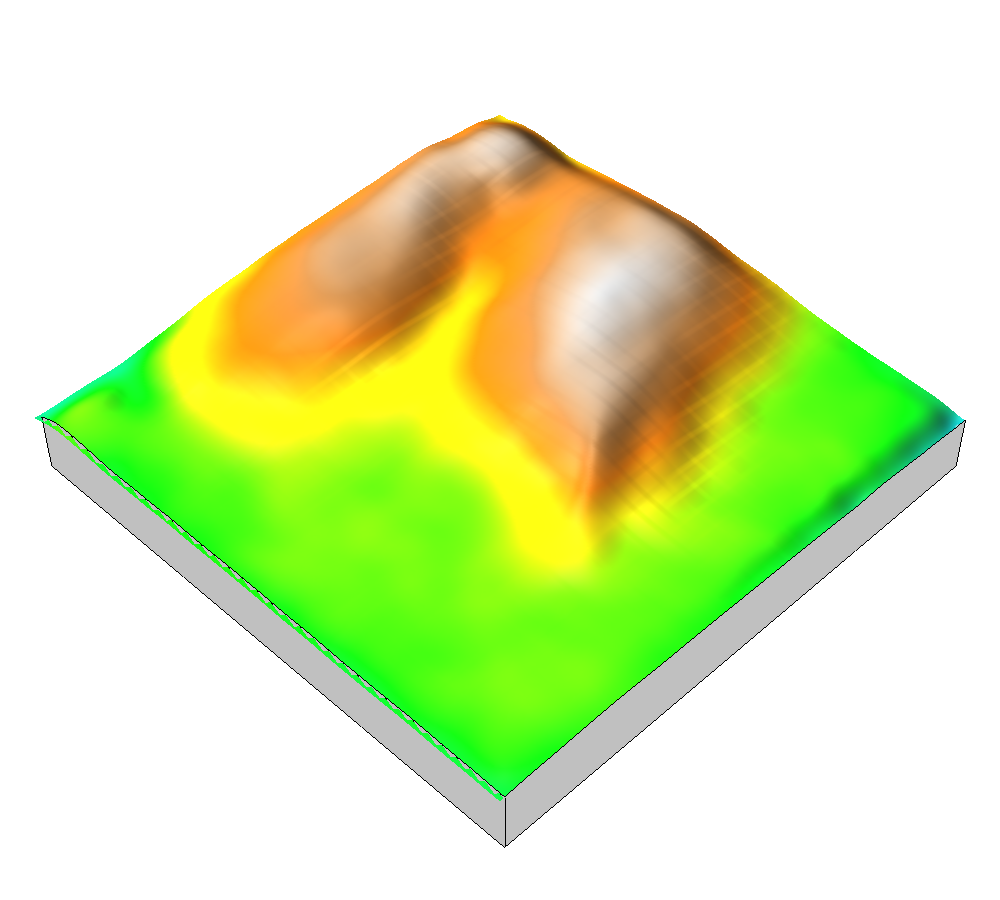
\includegraphics[width=0.08\textwidth]{images/render_3d/professionals/mean_dem_2.png}
		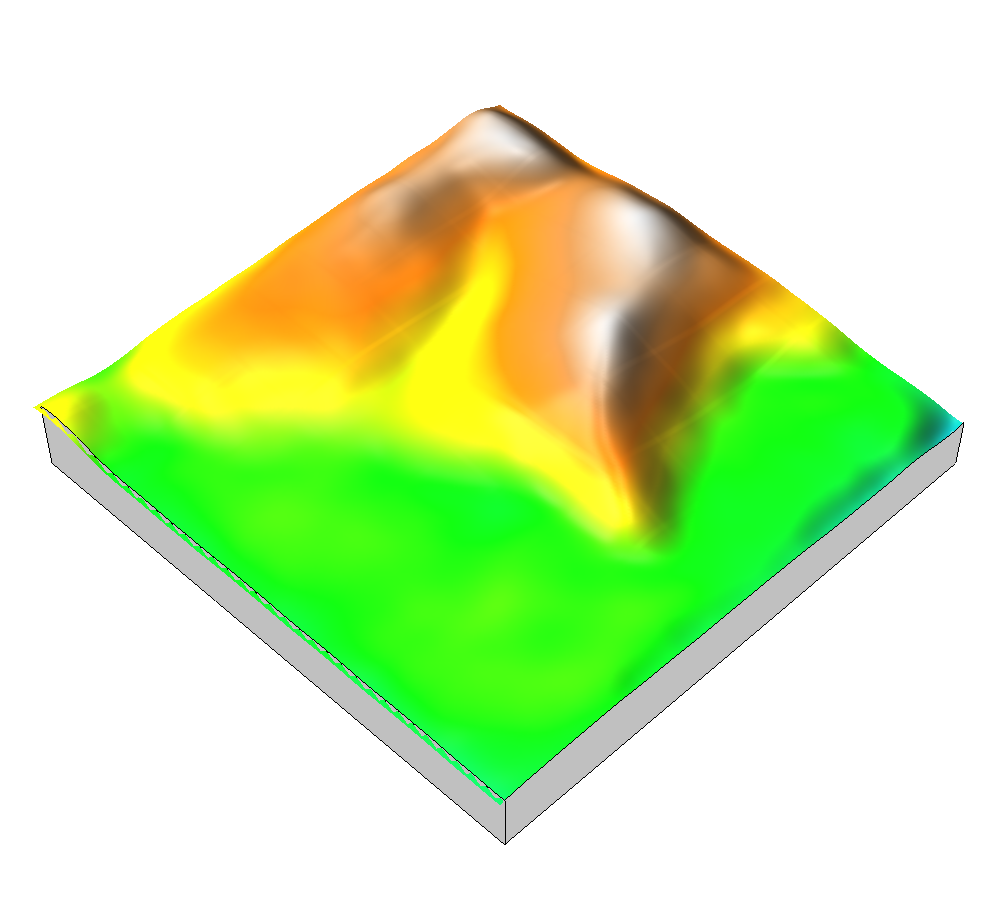
\includegraphics[width=0.08\textwidth]{images/render_3d/professionals/mean_dem_3.png}
		}
		child { node {3D novices \\ 
			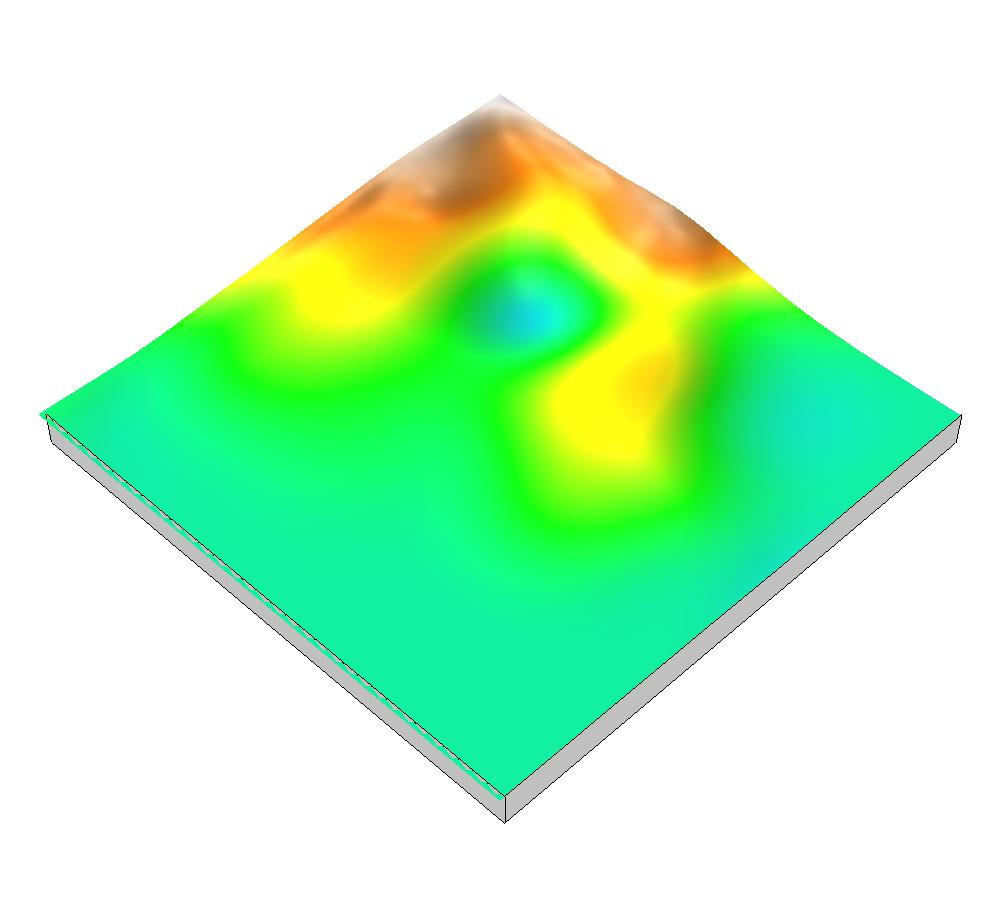
\includegraphics[width=0.08\textwidth]{images/render_3d/3d_novices/mean_dem_1.png}
			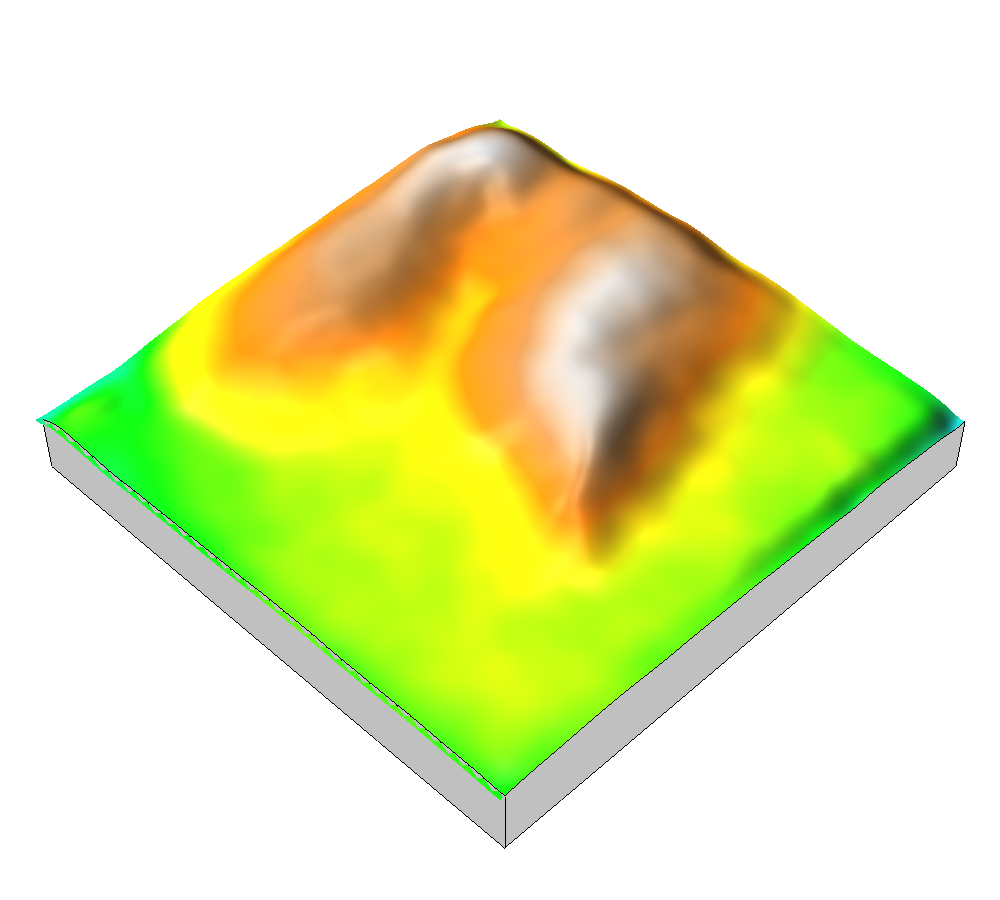
\includegraphics[width=0.08\textwidth]{images/render_3d/3d_novices/mean_dem_2.png}
			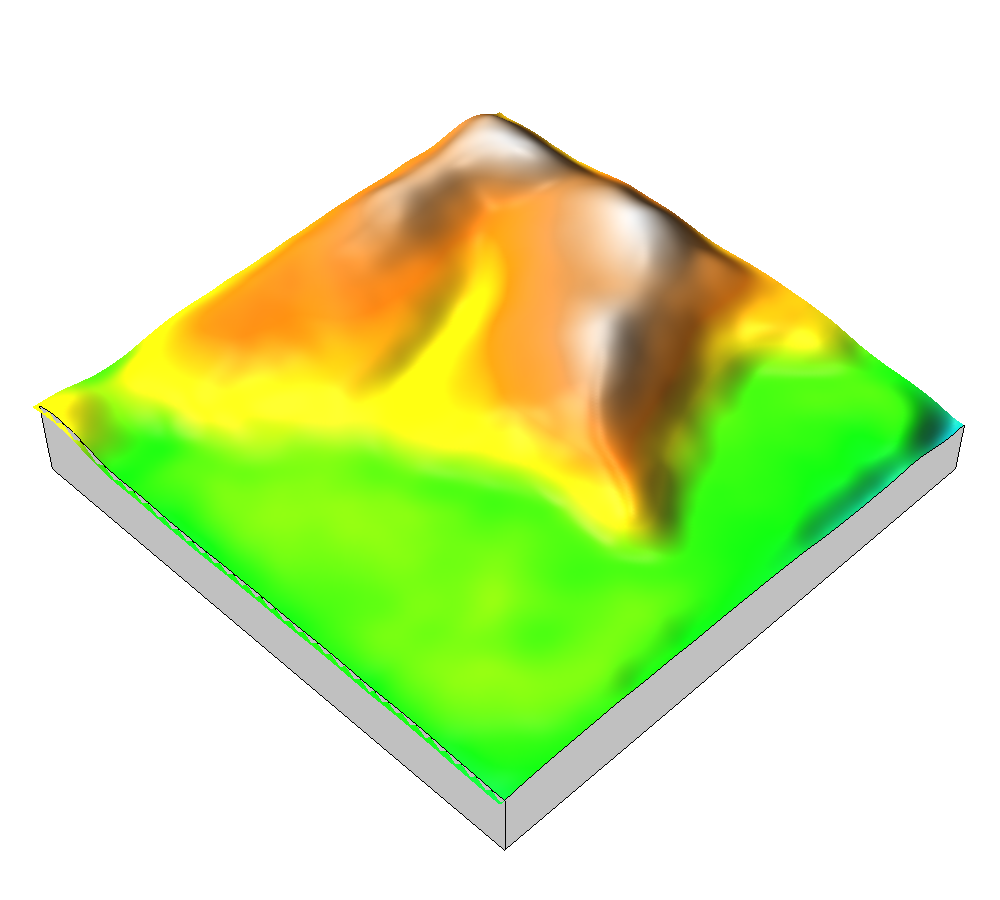
\includegraphics[width=0.08\textwidth]{images/render_3d/3d_novices/mean_dem_3.png}
			}
			}
		child { node {3D experts \\ 
			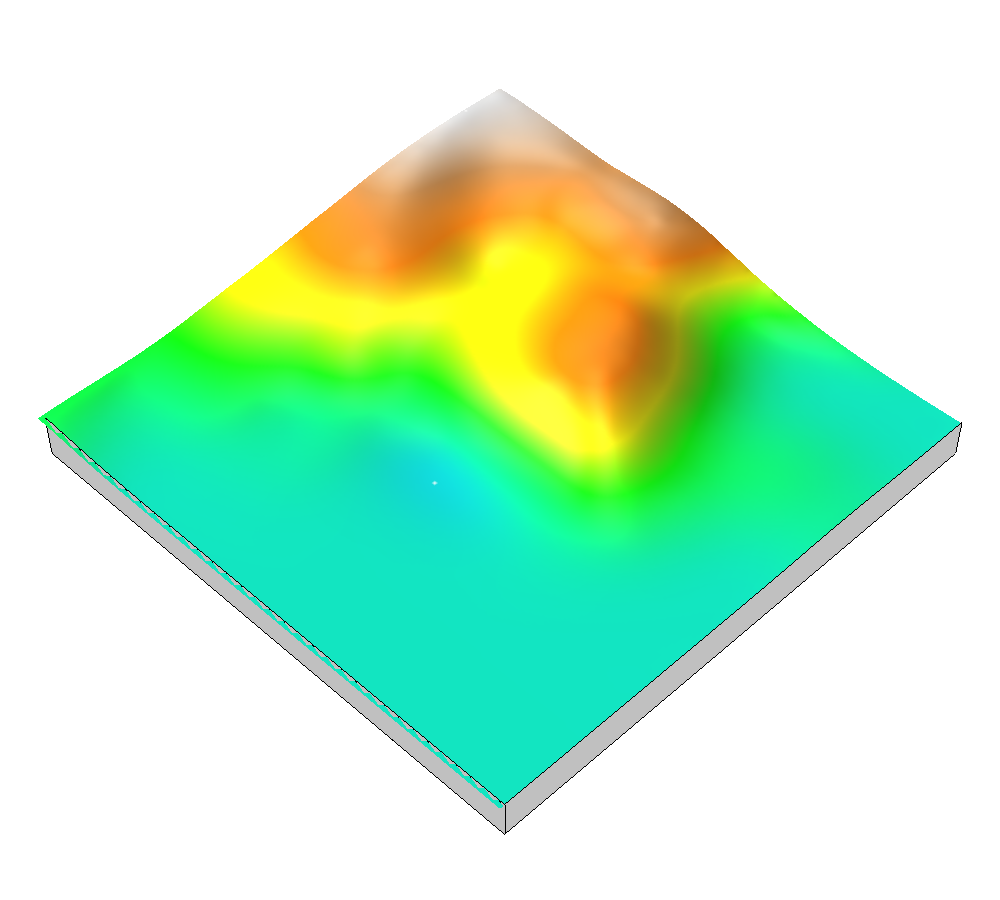
\includegraphics[width=0.08\textwidth]{images/render_3d/3d_experts/mean_dem_1.png}
			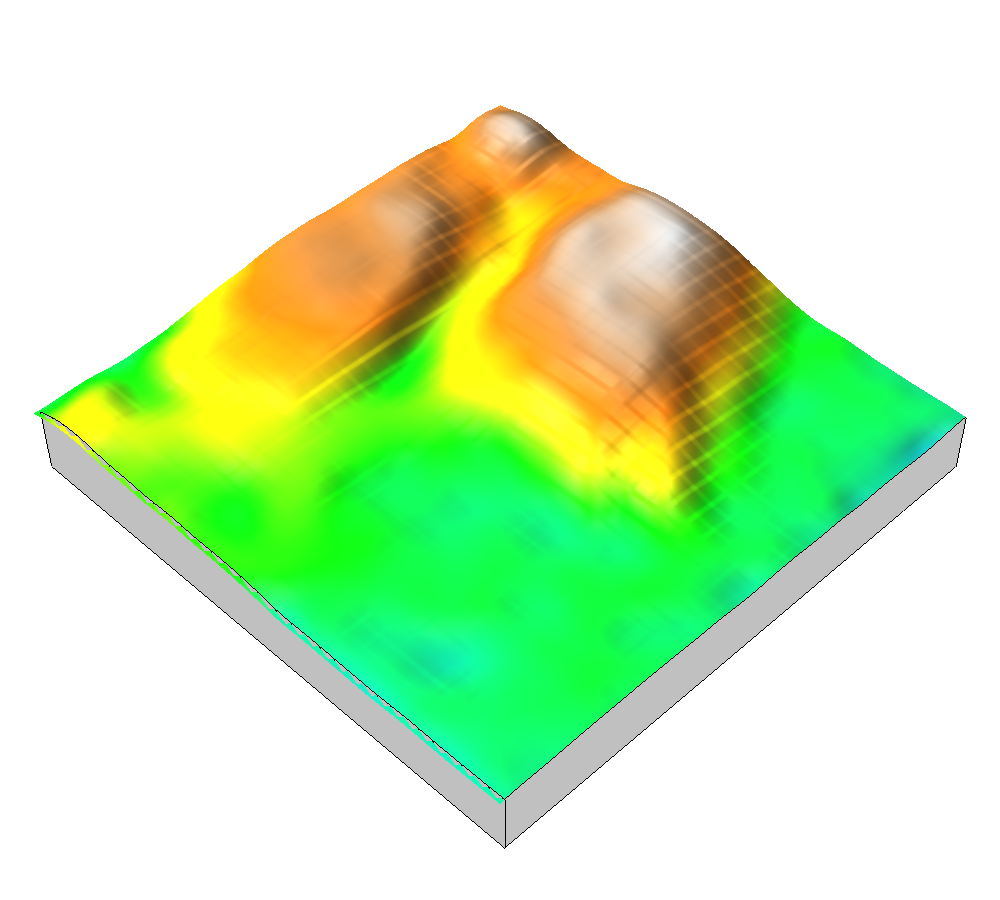
\includegraphics[width=0.08\textwidth]{images/render_3d/3d_experts/mean_dem_2.png}
			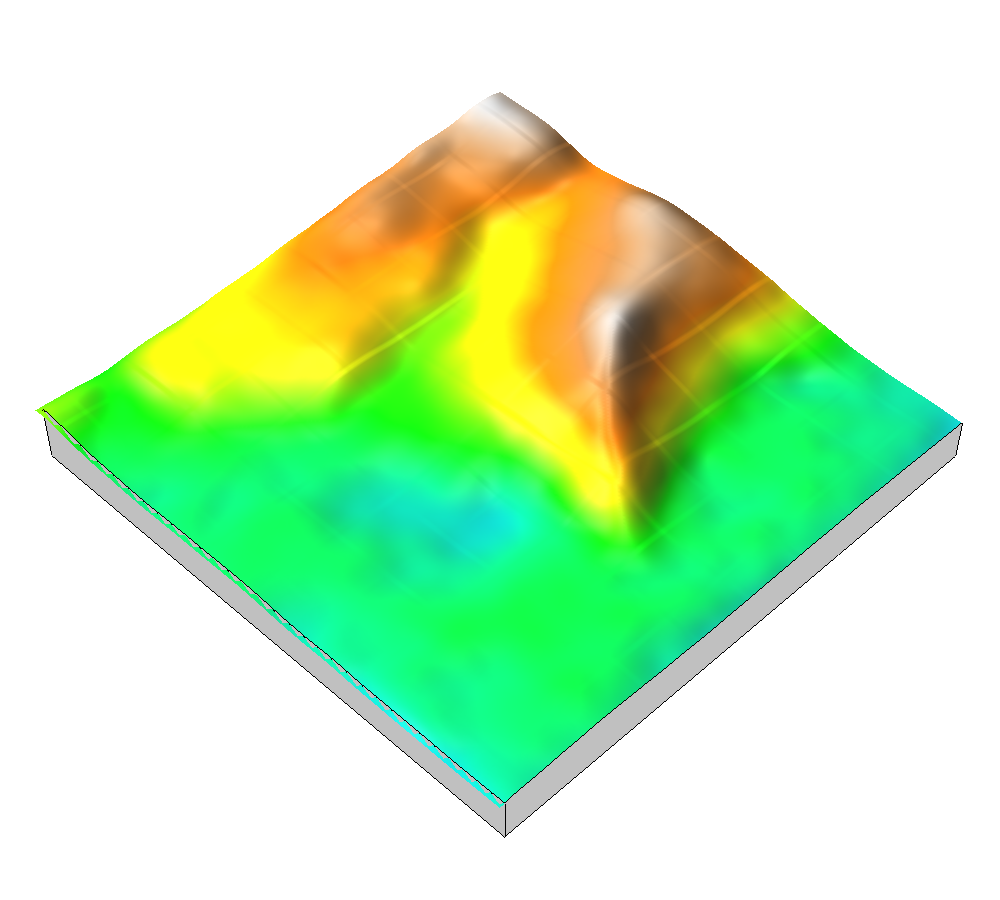
\includegraphics[width=0.08\textwidth]{images/render_3d/3d_experts/mean_dem_3.png}
			}
			}
};
\end{tikzpicture}
}
%
\caption{Pairwise comparison of the mean digital elevation models by category of participants}
\label{fig:tree}
\end{center}
\end{figure*}

% ---------------------------- TOPOGRAPHY ---------------------------- 
\begin{table*}[h]
\small\sf\centering
\caption{Topographic experiment: maps of per-cell statistics and geospatial analyses draped over 3D topography for all participants}
\ra{1.3}
\begin{tabular}{m{0.16\textwidth} m{0.18\textwidth} m{0.18\textwidth} m{0.18\textwidth} m{0.18\textwidth}}
\toprule
& \multicolumn{1}{c}{Reference} & \multicolumn{1}{c}{Digital} & \multicolumn{1}{c}{Analog}  & \multicolumn{1}{c}{Tangible}\\
\midrule
%
Mean elevation \par \vspace{0.5em} 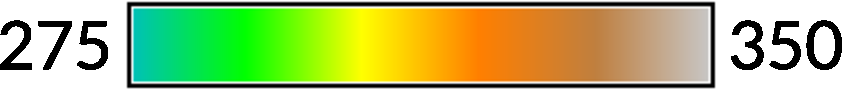
\includegraphics[width=0.16\textwidth]{images/legends/elevation_legend_1.pdf} & 
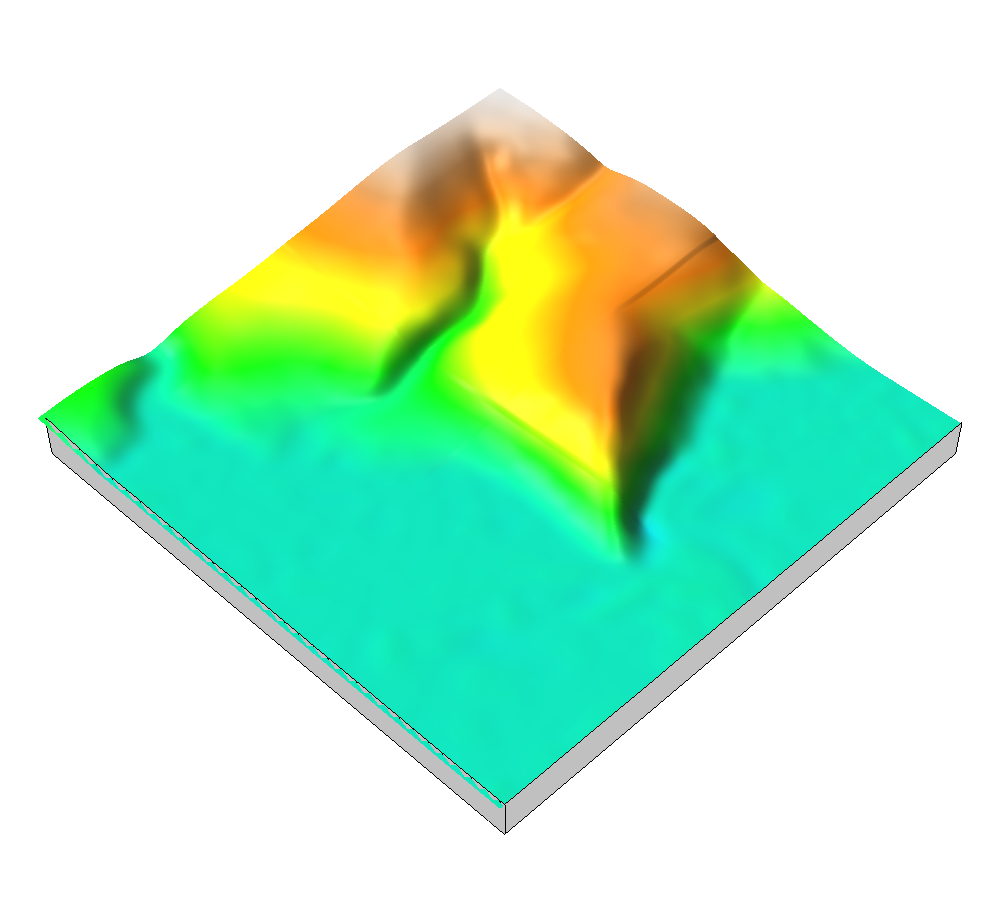
\includegraphics[width=0.18\textwidth]{images/render_3d/participants/dem_1.png} &
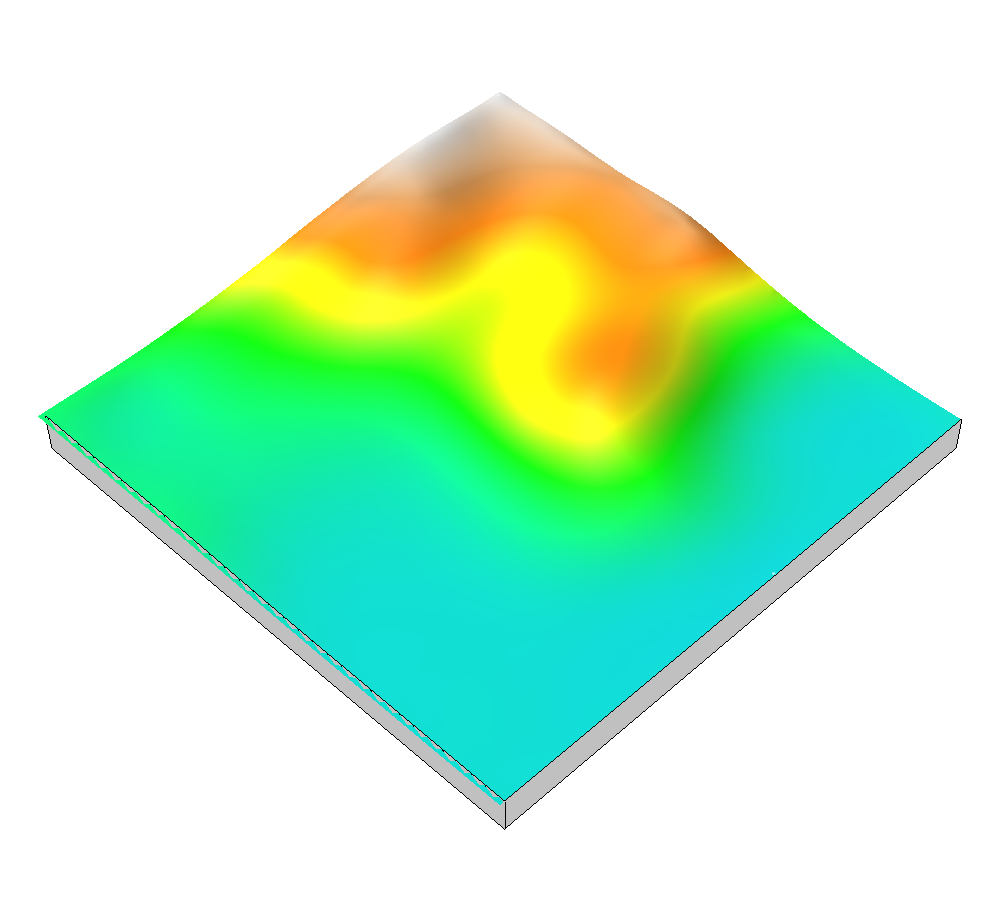
\includegraphics[width=0.18\textwidth]{images/render_3d/participants/mean_dem_1.png} &
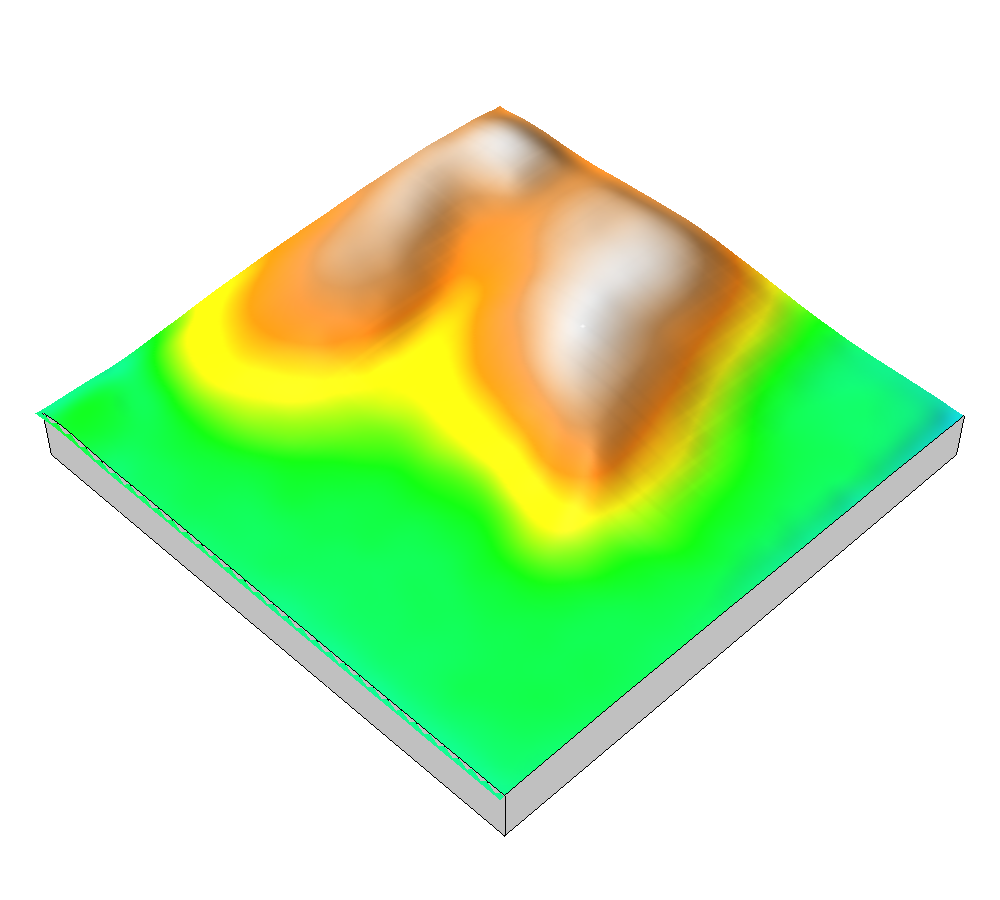
\includegraphics[width=0.18\textwidth]{images/render_3d/participants/mean_dem_2.png} &
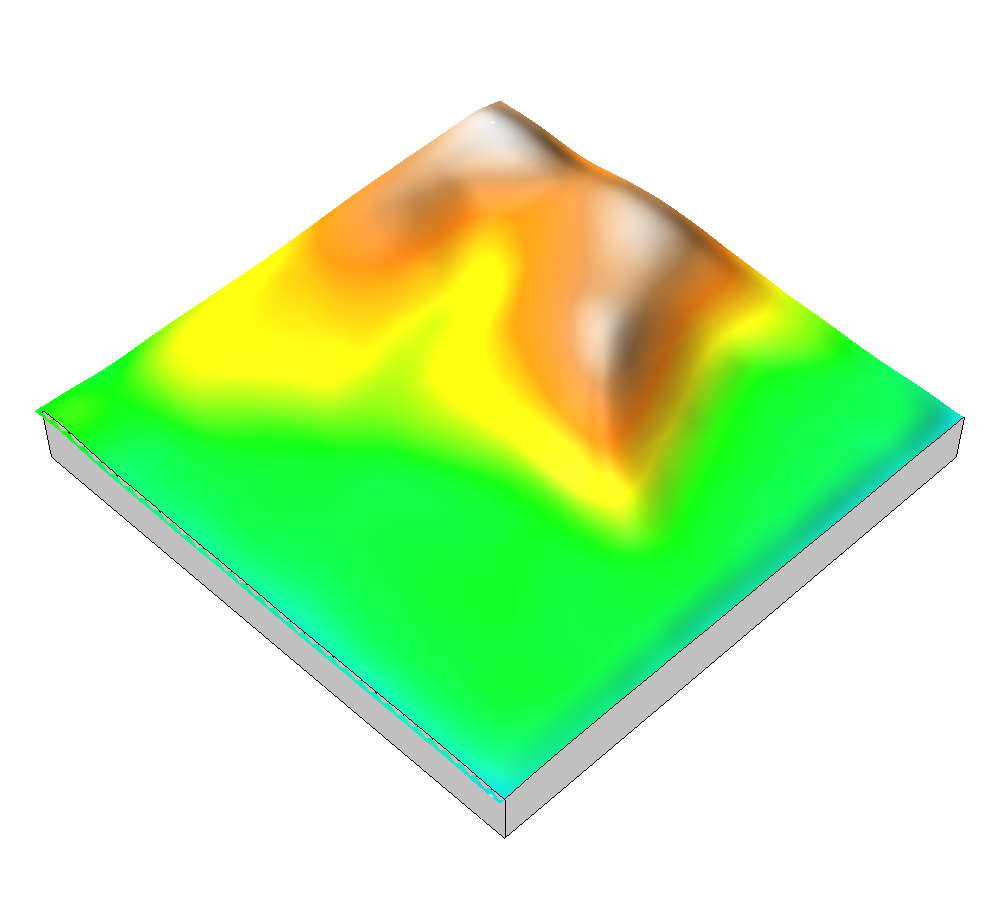
\includegraphics[width=0.18\textwidth]{images/render_3d/participants/mean_dem_3.png}\\
%
Stdev.~of elevations \par \vspace{0.5em} 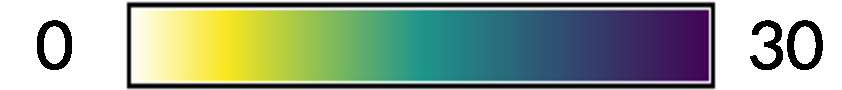
\includegraphics[width=0.16\textwidth]{images/legends/stdev_legend.pdf} & 
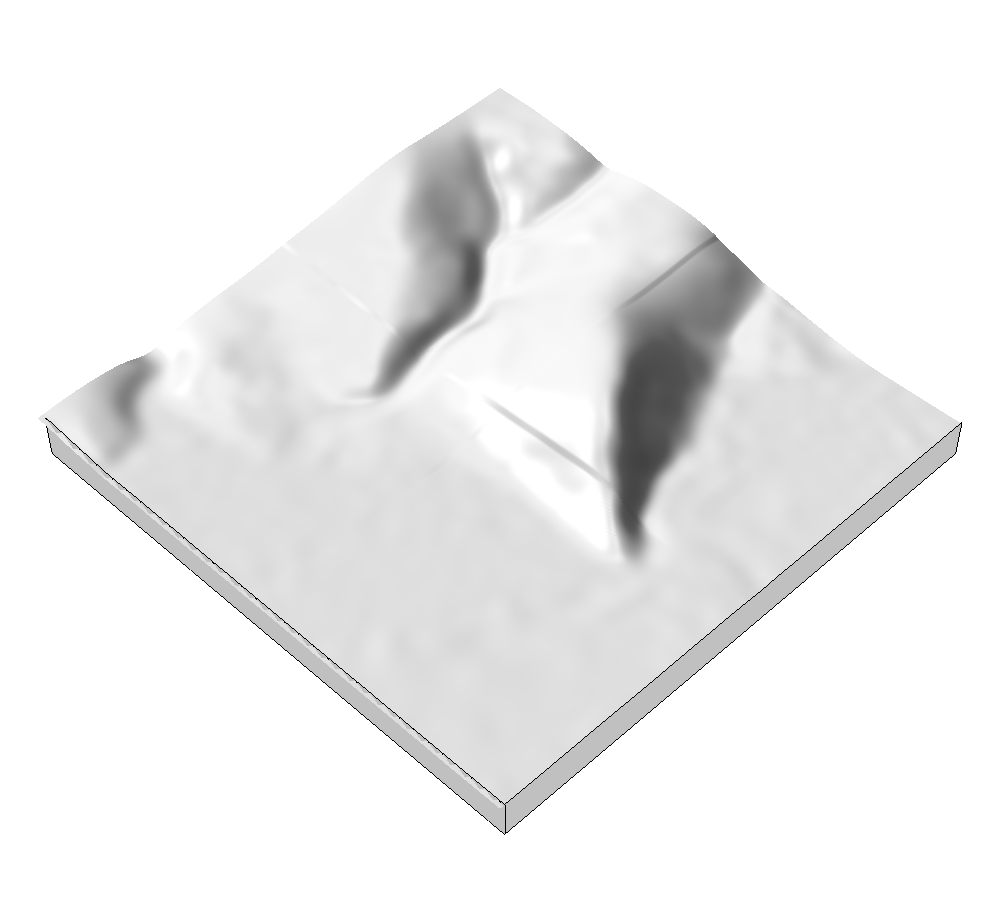
\includegraphics[width=0.18\textwidth]{images/render_3d/participants/dem_difference_1.png} &
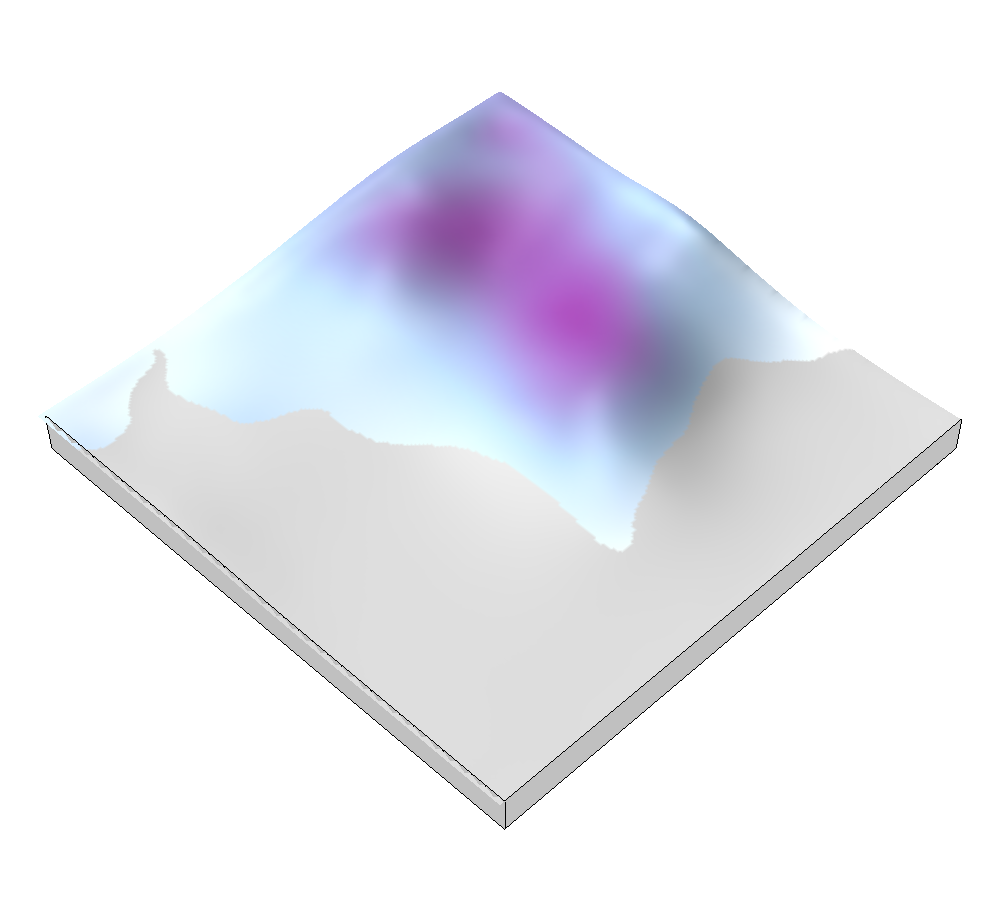
\includegraphics[width=0.18\textwidth]{images/render_3d/participants/stdev_dem_1.png} &
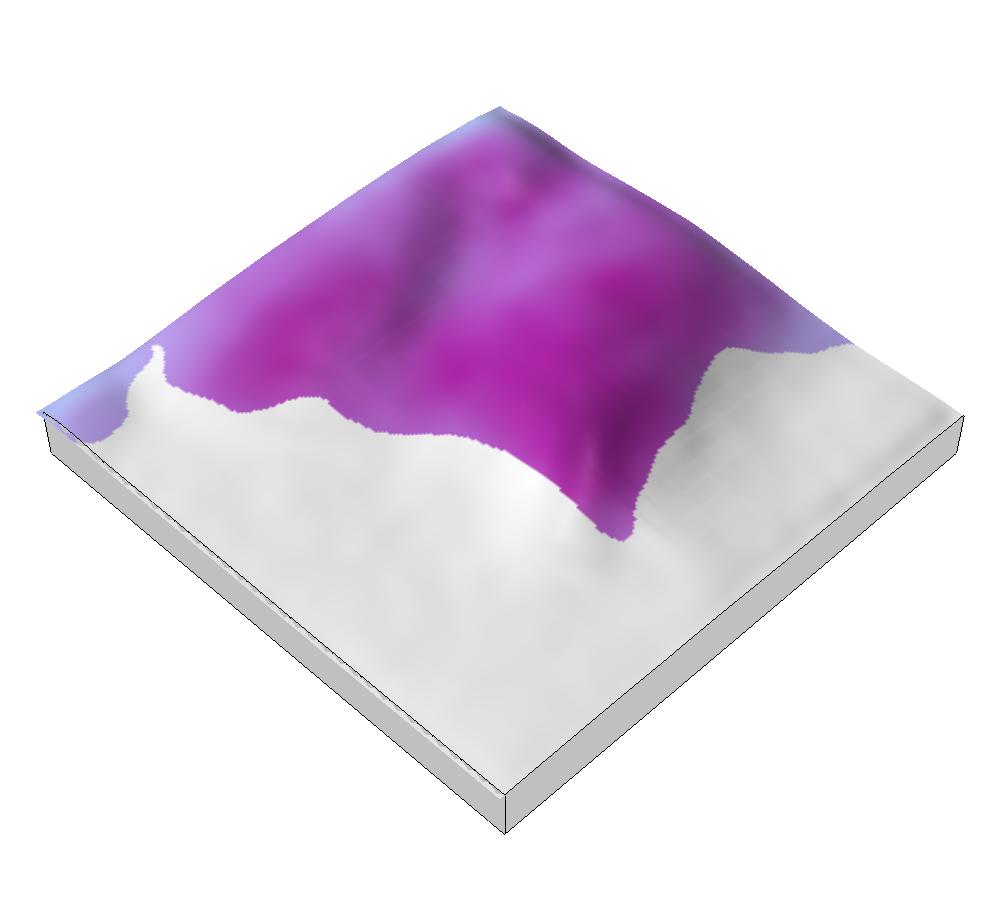
\includegraphics[width=0.18\textwidth]{images/render_3d/participants/stdev_dem_2.png} &
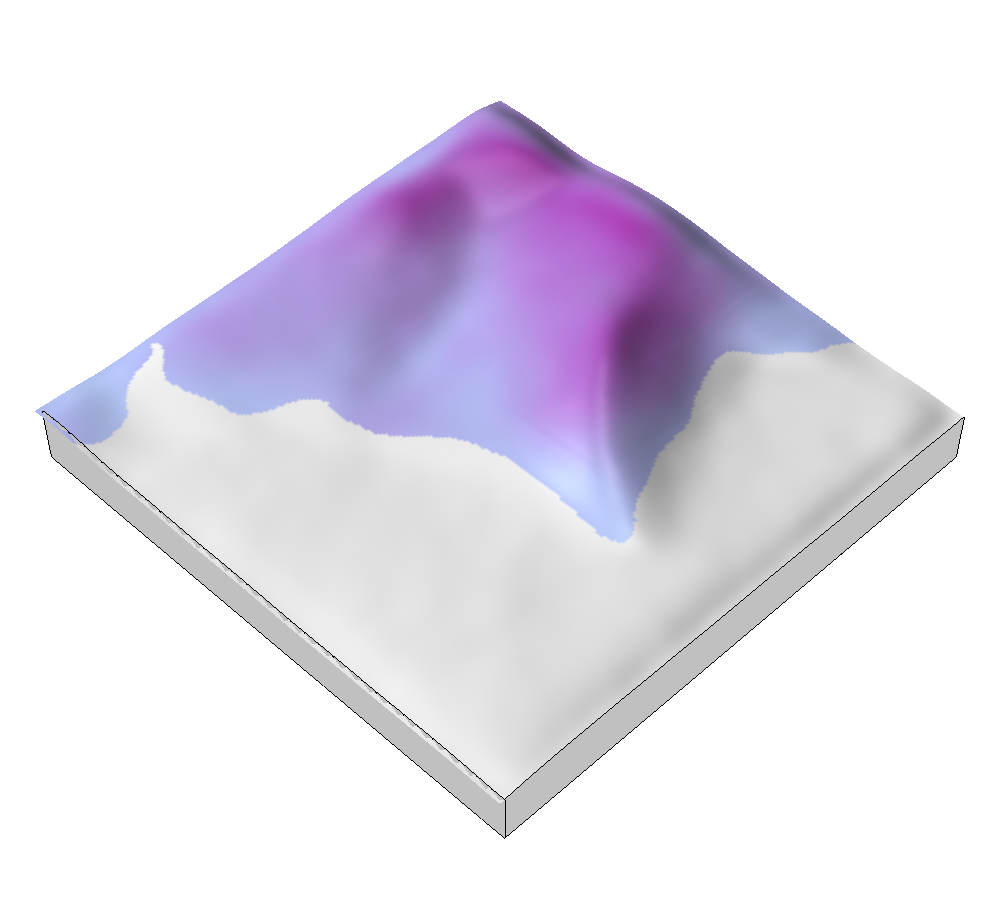
\includegraphics[width=0.18\textwidth]{images/render_3d/participants/stdev_dem_3.png}\\
%
Stdev.~of difference \par \vspace{0.5em} 
\includegraphics[width=0.16\textwidth]{images/legends/stdev_diff_legend.pdf} & 
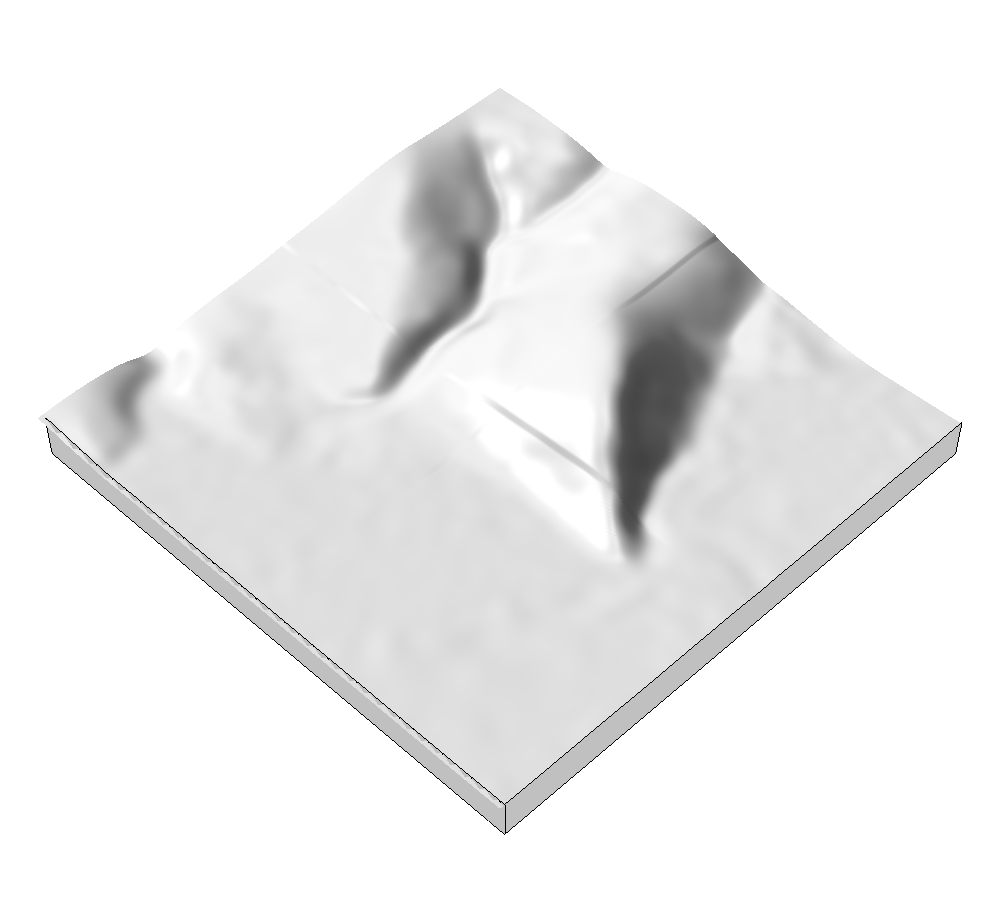
\includegraphics[width=0.18\textwidth]{images/render_3d/participants/dem_difference_1.png} &
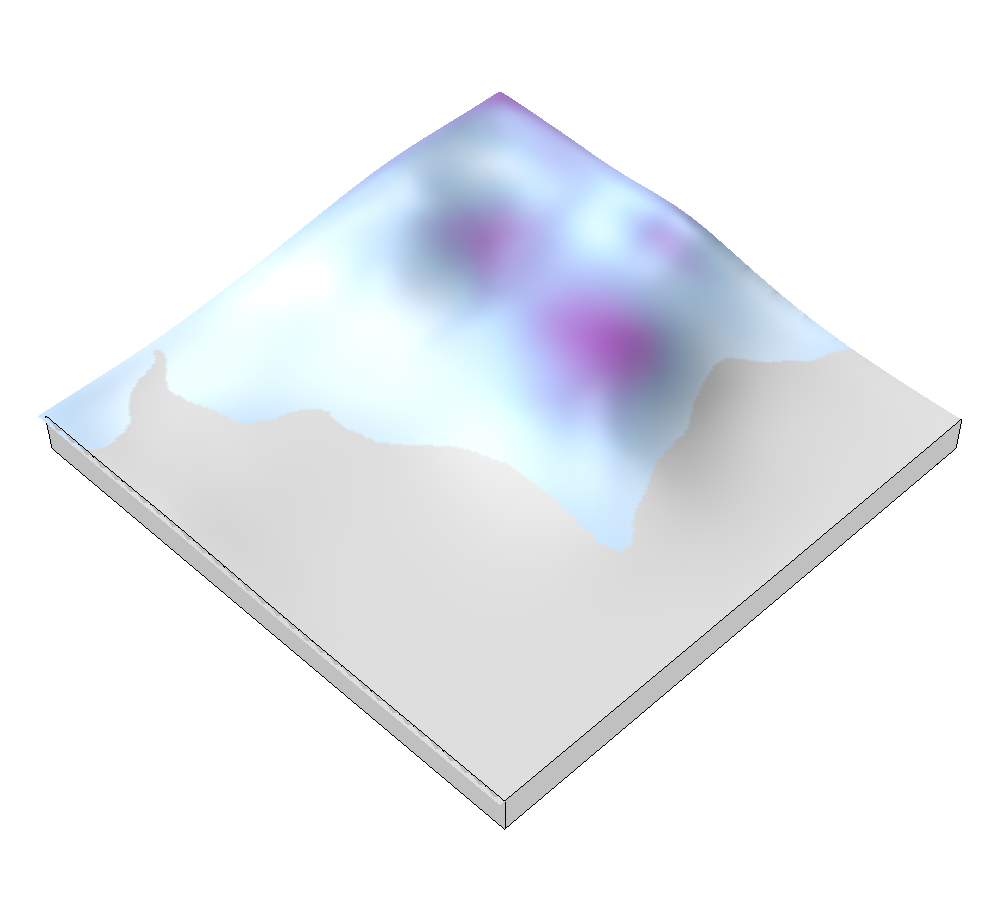
\includegraphics[width=0.18\textwidth]{images/render_3d/participants/stdev_regression_difference_series_1.png} &
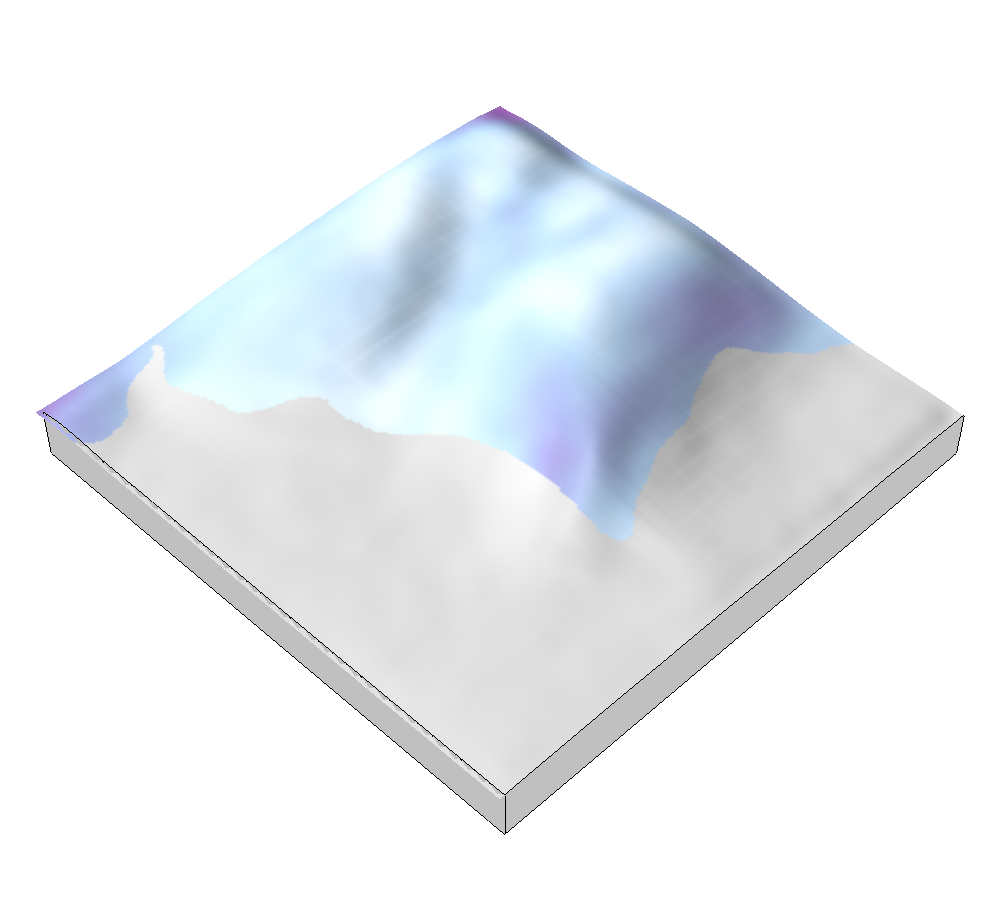
\includegraphics[width=0.18\textwidth]{images/render_3d/participants/stdev_regression_difference_series_2.png} &
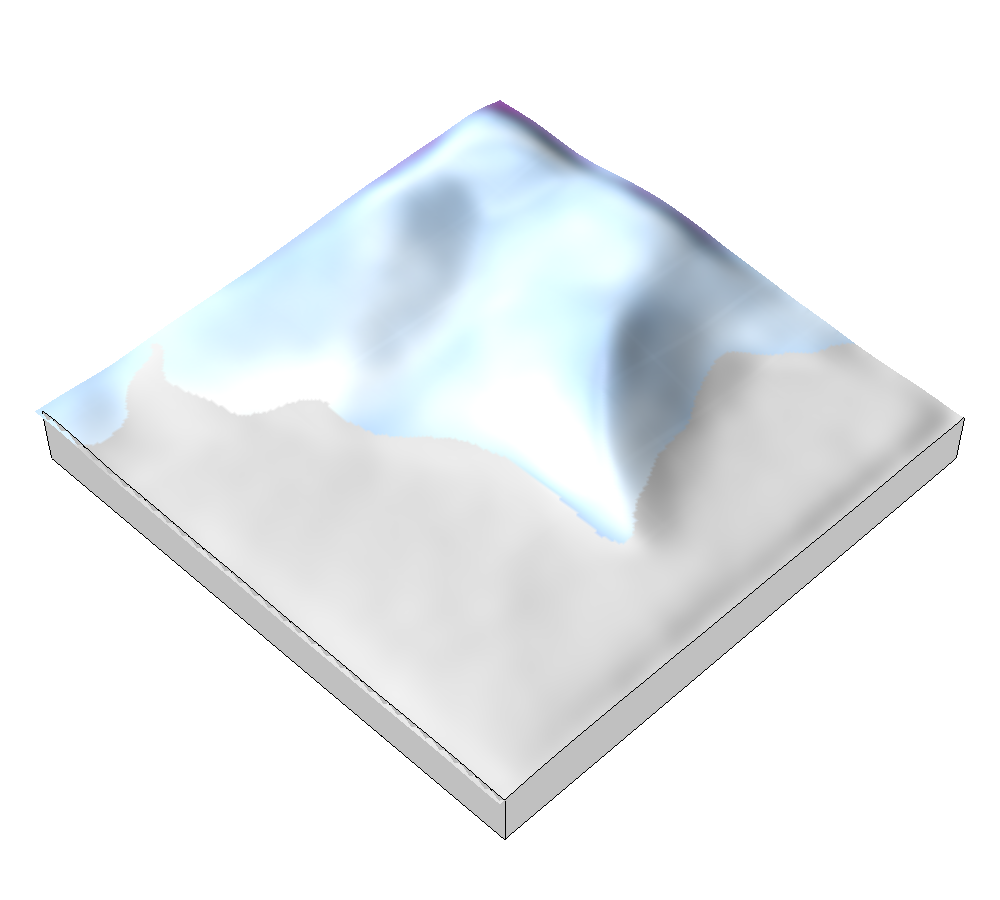
\includegraphics[width=0.18\textwidth]{images/render_3d/participants/stdev_regression_difference_series_3.png}\\
%
Mean difference \par \vspace{0.5em} 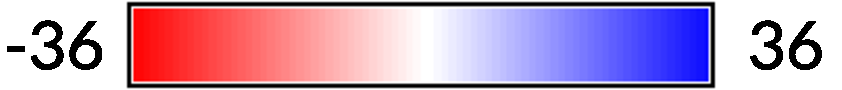
\includegraphics[width=0.16\textwidth]{images/legends/diff_legend.pdf} & 
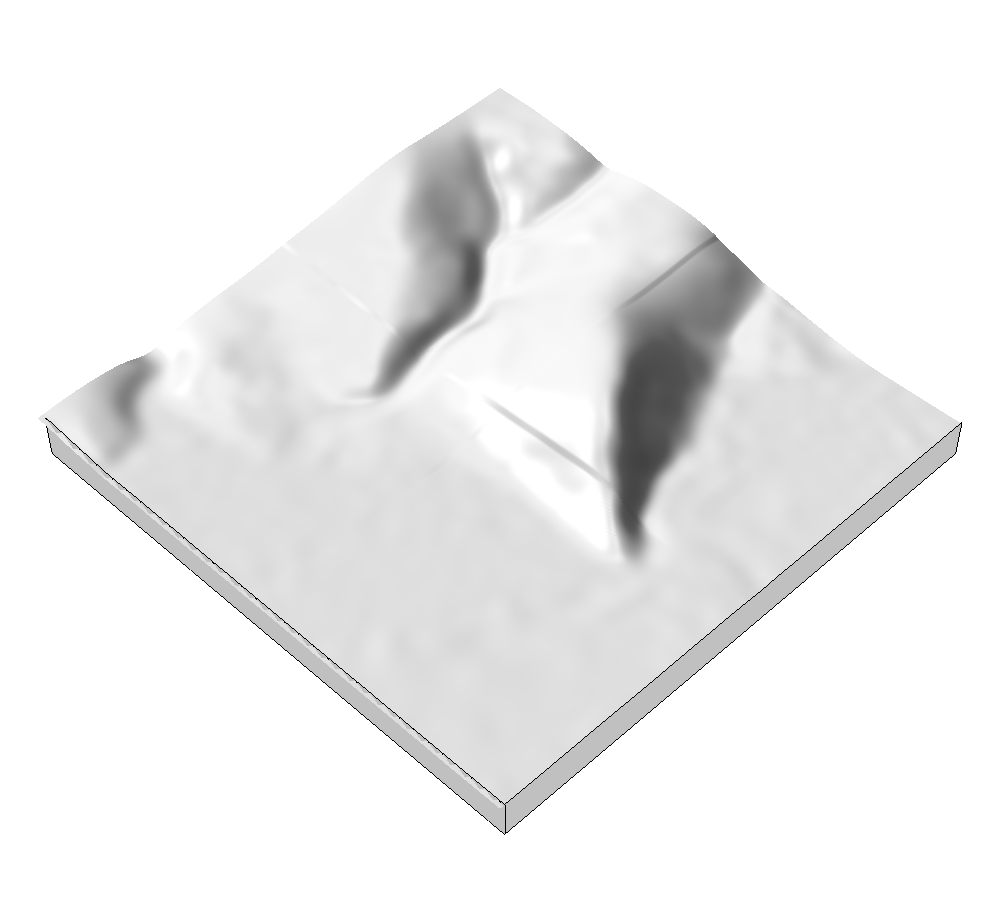
\includegraphics[width=0.18\textwidth]{images/render_3d/participants/dem_difference_1.png} &
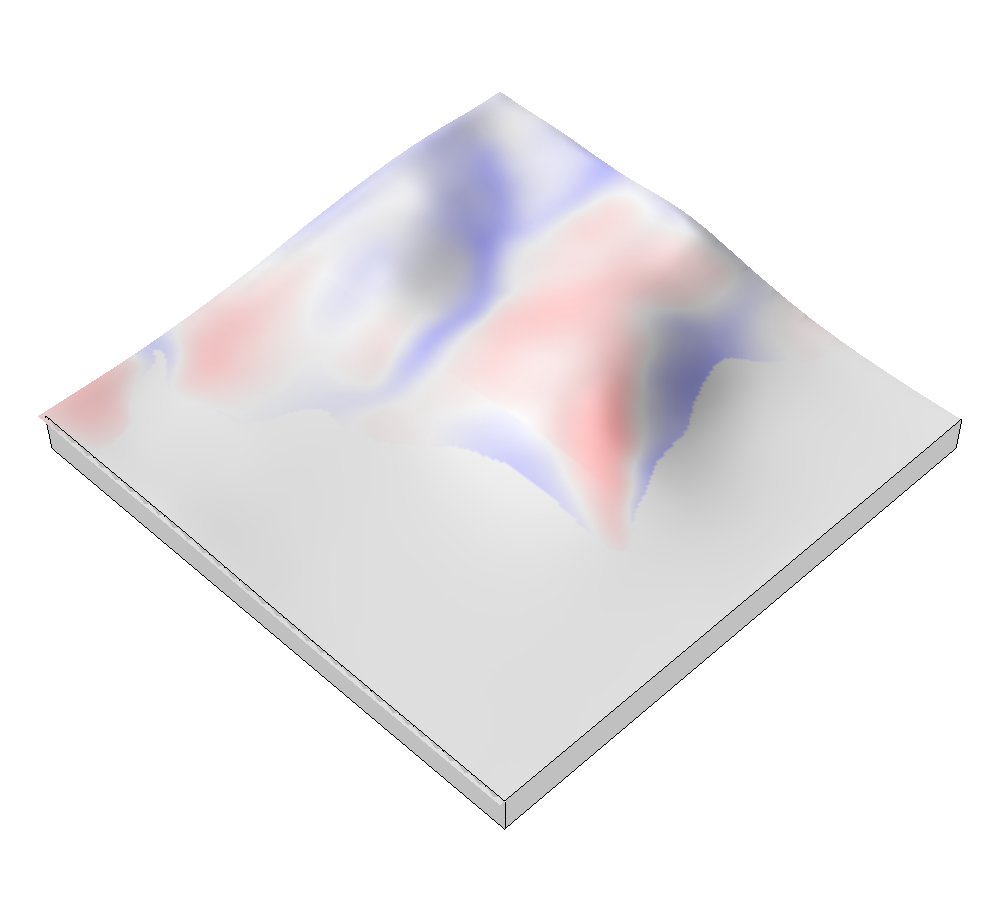
\includegraphics[width=0.18\textwidth]{images/render_3d/participants/mean_dem_regression_difference_1.png} &
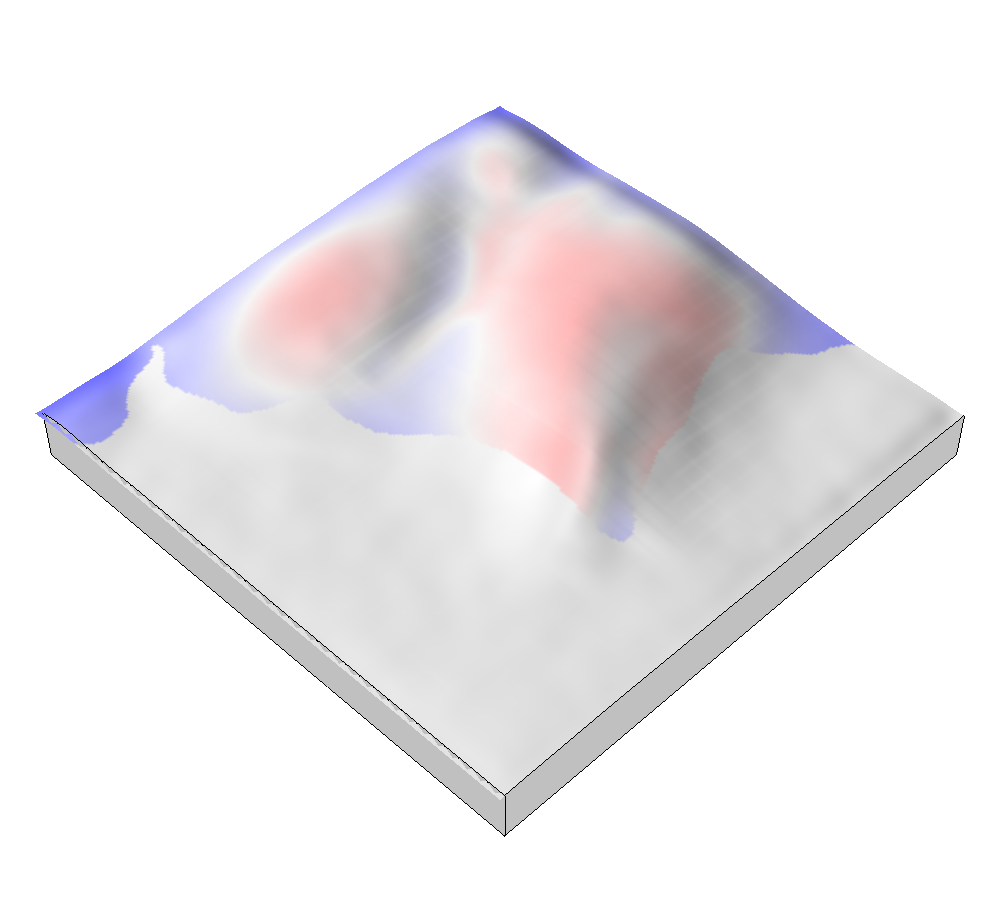
\includegraphics[width=0.18\textwidth]{images/render_3d/participants/mean_dem_regression_difference_2.png} &
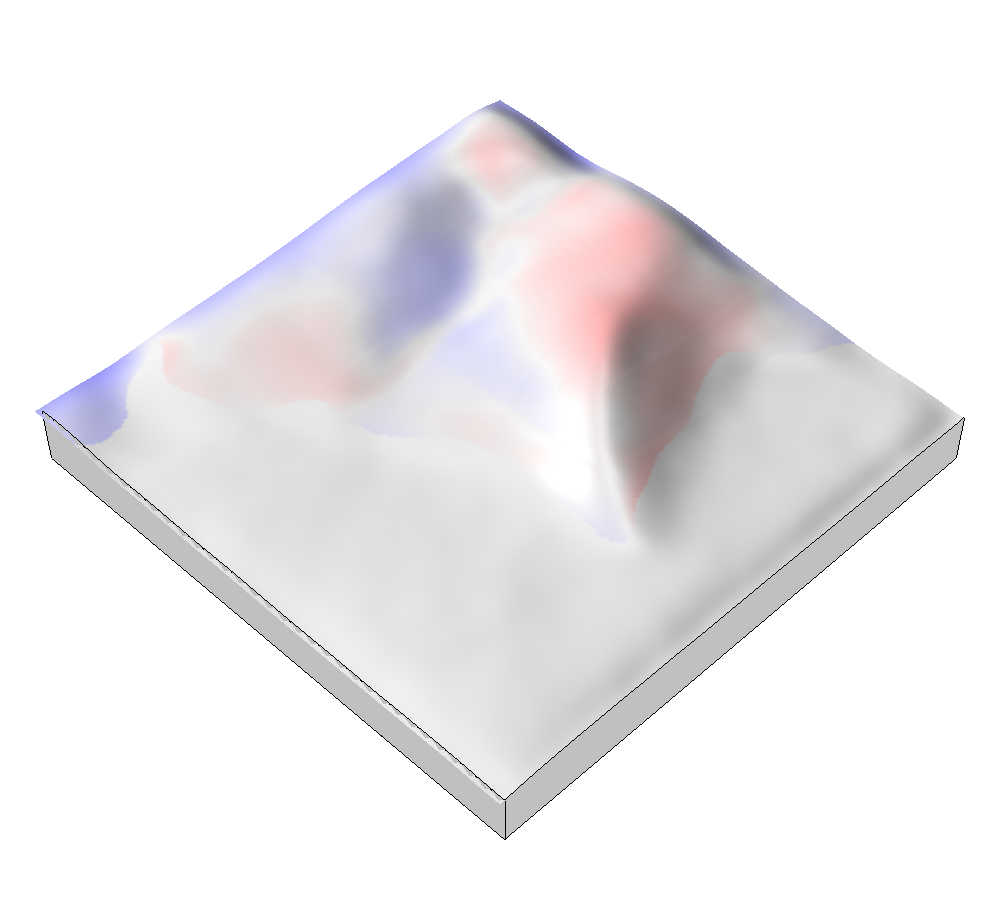
\includegraphics[width=0.18\textwidth]{images/render_3d/participants/mean_dem_regression_difference_3.png}\\
%
Mean slope \par \vspace{0.5em} 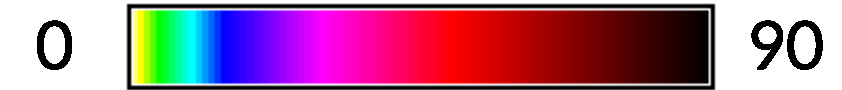
\includegraphics[width=0.16\textwidth]{images/legends/slope_legend.pdf} & 
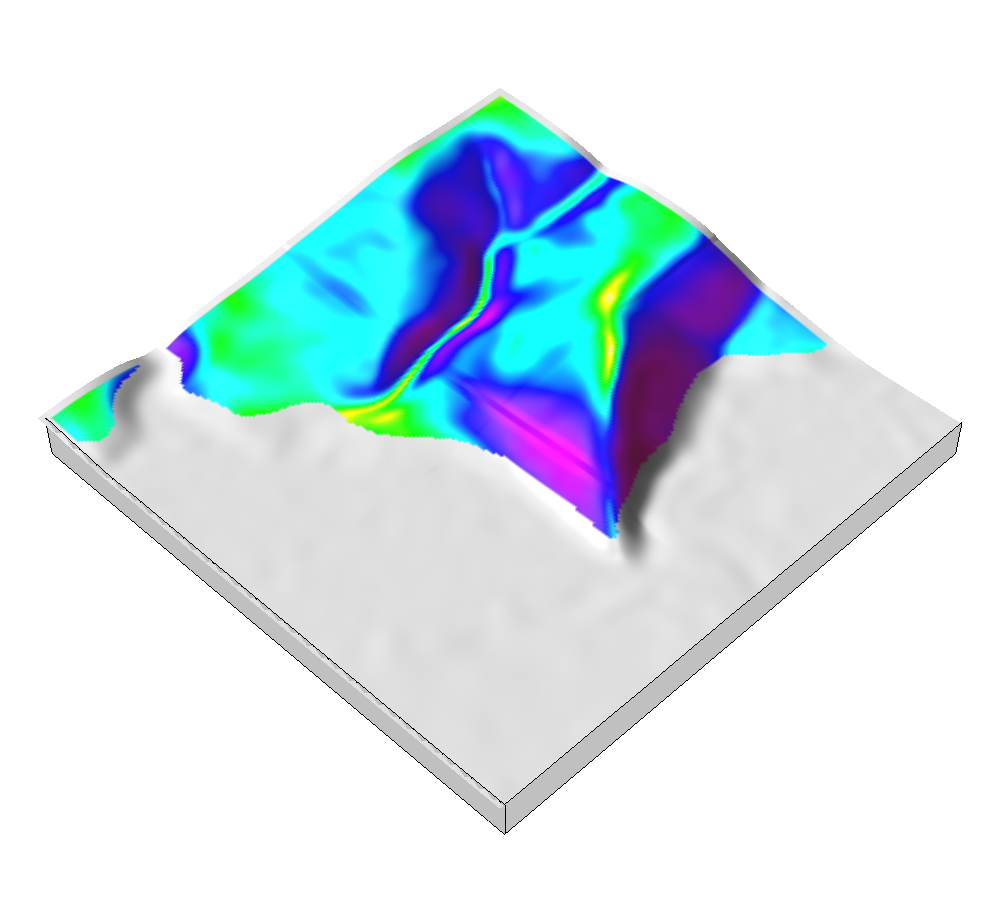
\includegraphics[width=0.18\textwidth]{images/render_3d/participants/slope_1.png} &
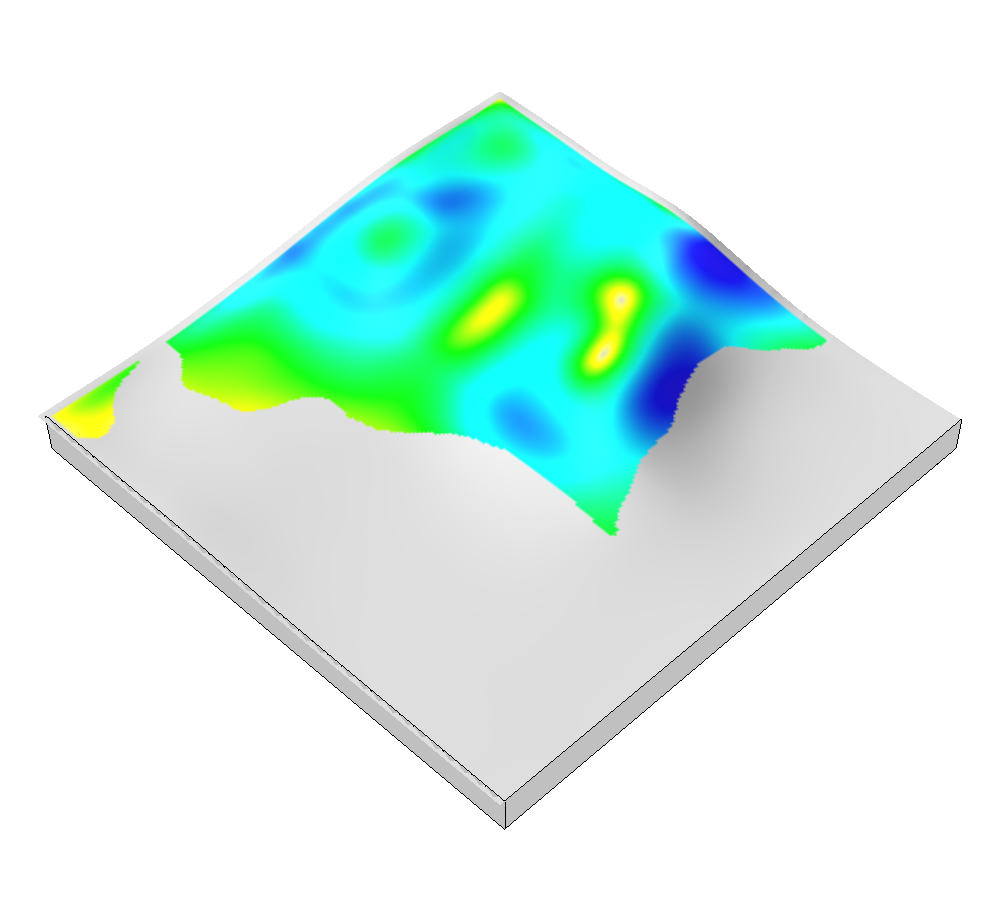
\includegraphics[width=0.18\textwidth]{images/render_3d/participants/mean_slope_1.png} &
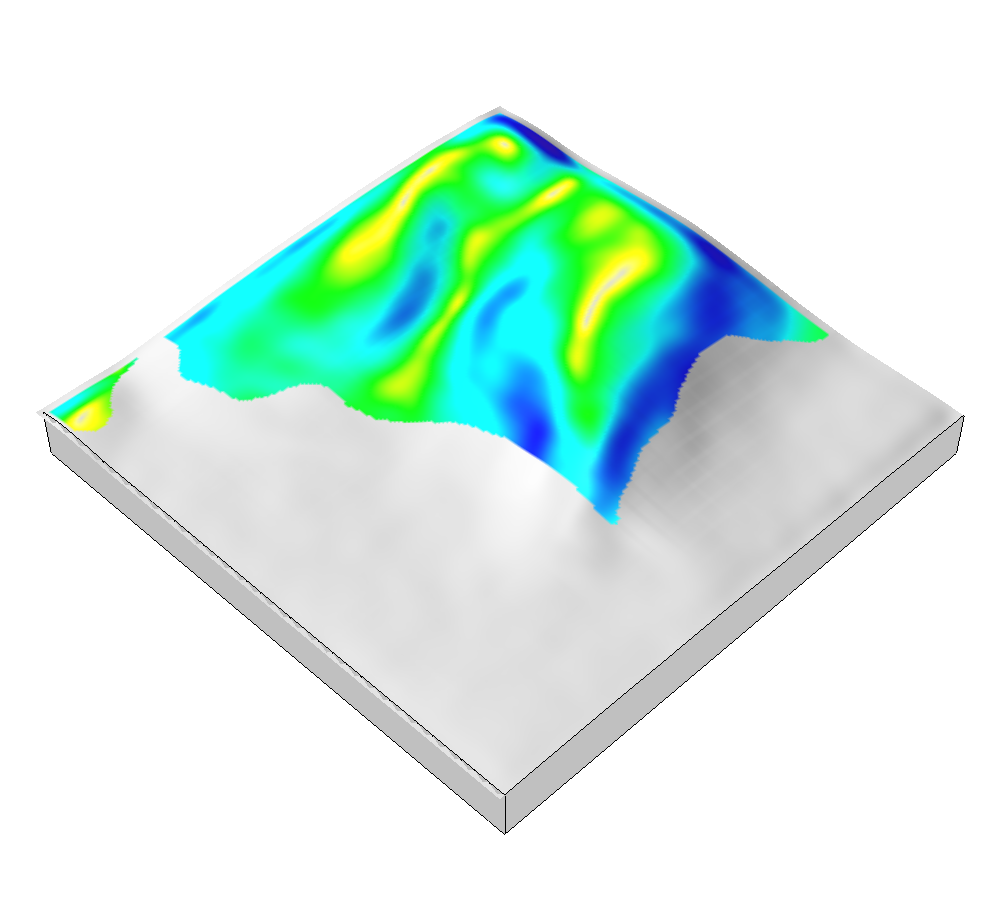
\includegraphics[width=0.18\textwidth]{images/render_3d/participants/mean_slope_2.png} &
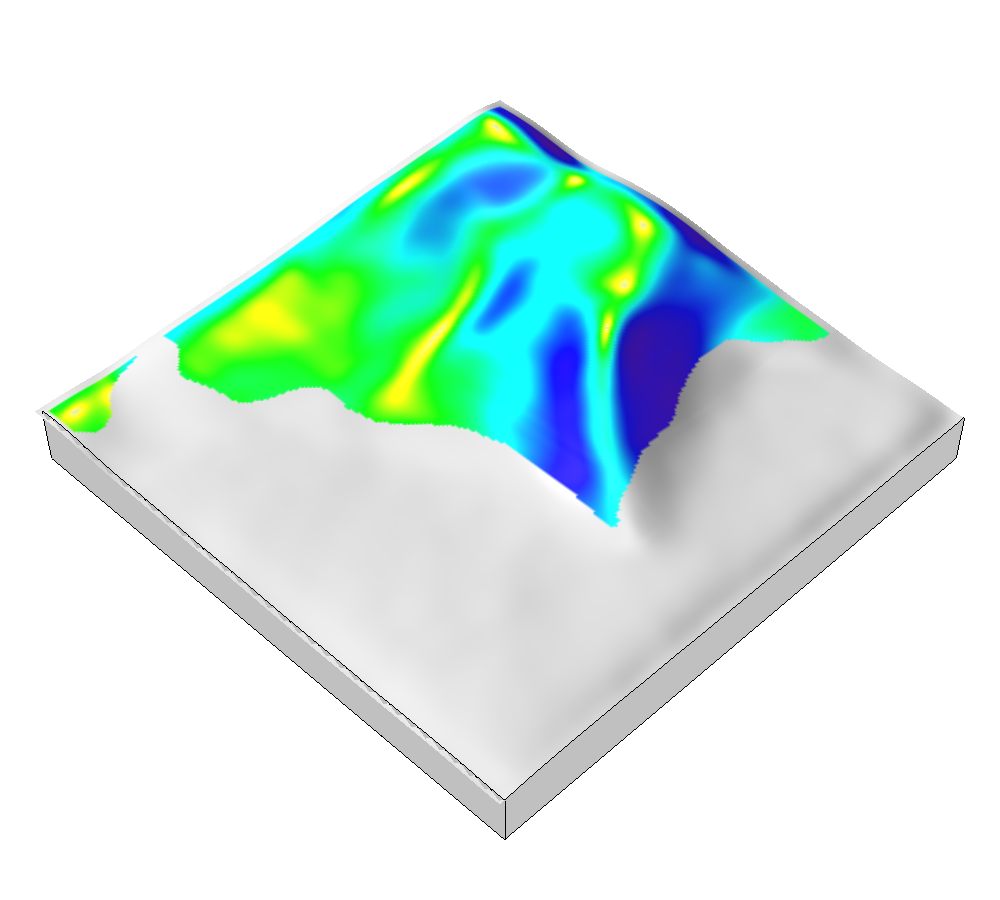
\includegraphics[width=0.18\textwidth]{images/render_3d/participants/mean_slope_3.png}\\
%
Mean landforms \par \vspace{0.5em} \includegraphics[width=0.16\textwidth]{images/legends/forms_legend.pdf} & 
\includegraphics[width=0.18\textwidth]{images/render_3d/participants/forms_1.png} &
\includegraphics[width=0.18\textwidth]{images/render_3d/participants/mean_forms_1.png} &
\includegraphics[width=0.18\textwidth]{images/render_3d/participants/mean_forms_2.png} &
\includegraphics[width=0.18\textwidth]{images/render_3d/participants/mean_forms_3.png}\\
%
\bottomrule
\end{tabular}
\label{table:topography}
%
\vspace*{1.5em}
%
\caption{Landforms identified by \textit{r.geomorphon}:
		1)~flat, 
		2)~peak, 
		3)~ridge, 
		4)~shoulder, 
		5)~spur, 
		6)~slope, 
		7)~hollow, 
		8)~footslope, 
		9)~valley, and
		10)~depression.
		Source: \cite{r.geomorphon}.}
\vspace*{1em}
\ra{1.3}
\begin{tabular}{m{0.6\textwidth}}
\includegraphics[width=0.6\textwidth]{images/geomorphons_legend.png}\\
\end{tabular}
\label{fig:geomorphons}
%
\end{table*}

% ---------------------------- DIFFERENCE ---------------------------- 

\begin{table*}[h]
\small\sf\centering
%
\caption{Cut-and-fill experiment: a participant sculpts the study landscape using Tangible Landscape's difference analytic, which shows where to add sand (blue) and remove sand (red).}
\vspace*{1em}
\ra{1.3}
\begin{tabular}{m{0.425\textwidth} m{0.425\textwidth}}
\includegraphics[width=0.425\textwidth]{images/experiments/difference_1.jpg} &
\includegraphics[width=0.425\textwidth]{images/experiments/difference_2.jpg}\\
\end{tabular}
\label{fig:diff} 
%
\vspace*{1.5em}
%
\caption{Cut-and-fill experiment: maps of per-cell statistics and geospatial analyses draped over a 3D rendering of the topography for all participants, 3D modeling novices, and 3D modeling experts}
\vspace*{1em}
\ra{1.3}
\begin{tabular}{m{0.1\textwidth} m{0.2\textwidth} m{0.2\textwidth} m{0.2\textwidth} m{0.2\textwidth}}
\toprule
& \multicolumn{1}{c}{Elevation} & \multicolumn{1}{c}{Stdev.~ of differences} & \multicolumn{1}{c}{Slope} & \multicolumn{1}{c}{Landforms}\\
\midrule
%
Reference & 
\includegraphics[width=0.2\textwidth]{images/render_3d/3d_experts/dem_4.png} &
\includegraphics[width=0.2\textwidth]{images/render_3d/3d_experts/dem_difference_4.png}
&
\includegraphics[width=0.2\textwidth]{images/render_3d/3d_experts/slope_4.png} &
\includegraphics[width=0.2\textwidth]{images/render_3d/3d_experts/forms_4.png}\\
%
Mean & 
\includegraphics[width=0.2\textwidth]{images/render_3d/participants/mean_dem_4.png} &
\includegraphics[width=0.2\textwidth]{images/render_3d/participants/stdev_regression_difference_series_4.png} &
\includegraphics[width=0.2\textwidth]{images/render_3d/participants/mean_slope_4.png} &
\includegraphics[width=0.2\textwidth]{images/render_3d/participants/mean_forms_4.png}\\
%
3D novices & 
\includegraphics[width=0.2\textwidth]{images/render_3d/3d_novices/mean_dem_4.png} &
\includegraphics[width=0.2\textwidth]{images/render_3d/3d_novices/stdev_regression_difference_series_4.png} &
\includegraphics[width=0.2\textwidth]{images/render_3d/3d_novices/mean_slope_4.png} &
\includegraphics[width=0.2\textwidth]{images/render_3d/3d_novices/mean_forms_4.png}\\
%
3D experts & 
\includegraphics[width=0.2\textwidth]{images/render_3d/3d_experts/mean_dem_4.png} &
\includegraphics[width=0.2\textwidth]{images/render_3d/3d_experts/stdev_regression_difference_series_4.png} &
\includegraphics[width=0.2\textwidth]{images/render_3d/3d_experts/mean_slope_4.png} &
\includegraphics[width=0.2\textwidth]{images/render_3d/3d_experts/mean_forms_4.png}\\
%
& 
\multicolumn{1}{c}{\includegraphics[width=0.2\textwidth]{images/legends/elevation_legend_4.pdf}} &
\multicolumn{1}{c}{\includegraphics[width=0.2\textwidth]{images/legends/stdev_diff_legend.pdf}} &
\multicolumn{1}{c}{\includegraphics[width=0.2\textwidth]{images/legends/slope_legend.pdf}} &
\multicolumn{1}{c}{\includegraphics[width=0.2\textwidth]{images/legends/forms_legend.pdf}}\\
%
\bottomrule
\end{tabular}
\label{table:difference_comparison}
%
\vspace*{1.5em}
%
\caption{Cut-and-fill experiment: percent cells}
\ra{1.3}
\begin{tabularx}{\textwidth}{YYYYYYYYYY}\toprule
Method && \multicolumn{2}{c}{Concentrated flow} & \phantom{abc}& \multicolumn{2}{c}{Ridges} &
\phantom{abc} & \multicolumn{2}{c}{Valleys}\\
\cmidrule{3-4} \cmidrule{6-7} \cmidrule{9-10}
&& Reference & Mean && Reference & Mean && Reference & Mean\\ \midrule
Difference && 1.94 & 0.90 && 4.27 & 2.93 && 2.96 & 0.13\\
\bottomrule
\end{tabularx}
\label{table:difference_percent_cells} 
%
\end{table*}

% ---------------------------- WATER FLOW ---------------------------- 

\begin{table*}[h]
\small\sf\centering
%
\caption{Water flow experiment: A participant sculpts the study landscape using Tangible Landscape's water flow analytic.}
\vspace*{1em}
\ra{1.3}
\begin{tabular}{m{0.5\textwidth}}
\includegraphics[width=0.5\textwidth]{images/experiments/tl_water.jpg}\\
\end{tabular}
\label{fig:flow_sequence} 
%
\vspace*{1.5em}
%
\caption{Water flow experiment: maps of of per-cell statistics and geospatial analyses draped over a 3D rendering of the topography for all participants, 3D modeling novices, and 3D experts}
\vspace*{1em}
\ra{1.3}
\begin{tabular}{m{0.1\textwidth} m{0.2\textwidth} m{0.2\textwidth} m{0.2\textwidth} m{0.2\textwidth}}
\toprule
& \multicolumn{1}{c}{Elevation} & \multicolumn{1}{c}{Stdev.~ of differences} & \multicolumn{1}{c}{Water depth} & \multicolumn{1}{c}{Depth difference}\\
\midrule
%
Reference & 
\includegraphics[width=0.2\textwidth]{images/render_3d/3d_experts/dem_5.png} &
\includegraphics[width=0.2\textwidth]{images/render_3d/3d_experts/dem_difference_5.png}
&
\includegraphics[width=0.2\textwidth]{images/render_3d/3d_experts/depth_5.png} &
\includegraphics[width=0.2\textwidth]{images/render_3d/3d_experts/dem_difference_5.png}\\
%
Mean & 
\includegraphics[width=0.2\textwidth]{images/render_3d/participants/mean_dem_5.png} &
\includegraphics[width=0.2\textwidth]{images/render_3d/participants/stdev_regression_difference_series_5.png} &
\includegraphics[width=0.2\textwidth]{images/render_3d/participants/mean_depth_5.png} &
\includegraphics[width=0.2\textwidth]{images/render_3d/participants/mean_depth_difference_5.png}\\
%
3D novices & 
\includegraphics[width=0.2\textwidth]{images/render_3d/3d_novices/mean_dem_5.png} &
\includegraphics[width=0.2\textwidth]{images/render_3d/3d_novices/stdev_regression_difference_series_5.png} &
\includegraphics[width=0.2\textwidth]{images/render_3d/3d_novices/mean_depth_5.png} &
\includegraphics[width=0.2\textwidth]{images/render_3d/3d_novices/mean_depth_difference_5.png}\\
%
3D experts & 
\includegraphics[width=0.2\textwidth]{images/render_3d/3d_experts/mean_dem_5.png} &
\includegraphics[width=0.2\textwidth]{images/render_3d/3d_experts/stdev_regression_difference_series_5.png} &
\includegraphics[width=0.2\textwidth]{images/render_3d/3d_experts/mean_depth_5.png} &
\includegraphics[width=0.2\textwidth]{images/render_3d/3d_experts/mean_depth_difference_5.png}\\
%
& 
\multicolumn{1}{c}{\includegraphics[width=0.2\textwidth]{images/legends/elevation_legend_5.pdf}} &
\multicolumn{1}{c}{\includegraphics[width=0.2\textwidth]{images/legends/stdev_diff_legend.pdf}} &
\multicolumn{1}{c}{\includegraphics[width=0.2\textwidth]{images/legends/depth_legend.pdf}} &
\multicolumn{1}{c}{\includegraphics[width=0.2\textwidth]{images/legends/depth_diff_legend.pdf}}\\
%
\bottomrule
\end{tabular}
\label{table:water_flow_experiment} 
%
\vspace*{1.5em}
%
\caption{Water flow experiment: percent cells}
\ra{1.3}
\begin{tabularx}{\textwidth}{YYYYYYYYYY}\toprule
Method && \multicolumn{2}{c}{Concentrated flow} & \phantom{abc}& \multicolumn{2}{c}{Ridges} &
\phantom{abc} & \multicolumn{2}{c}{Valleys}\\
\cmidrule{3-4} \cmidrule{6-7} \cmidrule{9-10}
&& Reference & Mean && Reference & Mean && Reference & Mean\\ \midrule
\mbox{Water flow} && 3.28 & 2.26 && 1.18 & 2.99 && 4.77 & 3.70\\
\bottomrule
\end{tabularx}
\label{table:water_flow_percent_cells} 
\end{table*}

\end{document}
